\documentclass[11pt]{article}

\usepackage[margin=0.82in]{geometry}
\usepackage[T1]{fontenc}
\usepackage{lmodern}
\usepackage{microtype}
\usepackage{amsmath}
\usepackage{amssymb}
\usepackage{booktabs}
\usepackage{longtable}
\usepackage{tabularx}
\usepackage{array}
\usepackage{enumitem}
\usepackage{xcolor}
\usepackage{listings}
\usepackage{graphicx}
\usepackage{float}
\usepackage{tikz}
\usetikzlibrary{arrows.meta,positioning,fit,shapes.geometric}
\usepackage{hyperref}

\definecolor{navy}{HTML}{17365D}
\definecolor{blue}{HTML}{2F75B5}
\definecolor{lightblue}{HTML}{D9EAF7}
\definecolor{green}{HTML}{548235}
\definecolor{lightgreen}{HTML}{E2F0D9}
\definecolor{orange}{HTML}{C65911}
\definecolor{lightorange}{HTML}{FCE4D6}
\definecolor{red}{HTML}{C00000}
\definecolor{graybg}{HTML}{F3F5F7}
\definecolor{darkgray}{HTML}{404040}

\hypersetup{
  colorlinks=true,
  linkcolor=navy,
  urlcolor=blue,
  citecolor=navy,
  pdftitle={Prefix KV-Cache Policy Evolution: Simulator, Verifier, and Search Architecture}
}

\lstdefinestyle{python}{
  language=Python,
  basicstyle=\ttfamily\small,
  keywordstyle=\color{navy}\bfseries,
  commentstyle=\color{green},
  stringstyle=\color{orange},
  backgroundcolor=\color{graybg},
  frame=single,
  rulecolor=\color{lightblue},
  breaklines=true,
  showstringspaces=false,
  columns=fullflexible,
  keepspaces=true,
  xleftmargin=0.5em,
  xrightmargin=0.5em
}

\lstdefinestyle{shell}{
  language=bash,
  basicstyle=\ttfamily\small,
  backgroundcolor=\color{graybg},
  frame=single,
  rulecolor=\color{lightblue},
  breaklines=true,
  showstringspaces=false,
  columns=fullflexible,
  keepspaces=true
}

\newcommand{\code}[1]{\texttt{\detokenize{#1}}}
\newcommand{\filepath}[1]{\nolinkurl{#1}}
\newcommand{\identifier}[1]{\nolinkurl{#1}}
\newcommand{\metric}[1]{\texttt{\detokenize{#1}}}
\newcommand{\important}[1]{\textbf{\color{navy}#1}}
\newcommand{\risk}[1]{\textbf{\color{red}#1}}
\newcommand{\good}[1]{\textbf{\color{green}#1}}

\setlist[itemize]{leftmargin=1.35em,itemsep=0.25em,topsep=0.35em}
\setlist[enumerate]{leftmargin=1.55em,itemsep=0.25em,topsep=0.35em}
\setlength{\emergencystretch}{2em}
\setlength{\parindent}{0pt}
\setlength{\parskip}{0.55em}

\title{\textbf{\color{navy}Prefix KV-Cache Policy Evolution}\\
\large Supplementary Research Log and Negative Results}
\author{Experimental Record}
\date{June 9, 2026}

\begin{document}

\maketitle

\begin{abstract}
This supplementary document preserves the detailed experimental chronology, run-level
measurements, engineering journey, and rejected evolutionary solutions behind the
current system.  It is intentionally separated from the main technical report so that
\filepath{docs/technical_report.tex} can present the current method and evidence
without reading like a lab notebook.  Operative claims should be taken from the main
report and the generated summaries under \filepath{docs/results/}; historical scores
below are not necessarily comparable across verifier revisions.
\end{abstract}

\tableofcontents
\newpage

\section{How to Read This Record}

This document is evidence preservation, not the primary system specification.  It
retains detailed run narratives because failed searches, verifier changes, and
negative results explain why the current workflow has its present trust boundaries,
feedback channels, and promotion gates.  The main report cites only the conclusions
that remain relevant to the current design.

\section{Mutation-Operator Productivity}
\label{sec:operator-productivity}

The completed 500-budget function-only eviction-specialist run provides an unusually
clear diagnostic of Levi's punctuated-equilibrium design.  The final snapshot of run
\identifier{20260608_150431_280387} records 498 evaluations, four evaluation errors,
twenty scored seed or initialization entries, and 474 scored post-initialization
proposals.  Table~\ref{tab:operator-productivity} classifies those proposals by their
recorded sampler.  Acceptance means that a proposal entered or replaced a behavior-
archive cell; it does not mean that the proposal became the scalar incumbent.

\begin{table}[H]
\centering
\small
\begin{tabular}{lrrrrr}
\toprule
\textbf{Operator} & \textbf{Scored} & \textbf{Accepted} &
\textbf{Accept rate} & \textbf{New best} & \textbf{New-best rate} \\
\midrule
Normal GPT-5.4-mini mutation & 422 & 74 & \(17.5\%\) & 7 & \(1.7\%\) \\
GPT-5.4-mini PE variant & 39 & 4 & \(10.3\%\) & 3 & \(7.7\%\) \\
Direct GPT-5.5 paradigm shift & 13 & 5 & \(38.5\%\) & 3 & \(23.1\%\) \\
\bottomrule
\end{tabular}
\caption{Operator productivity in the completed eviction-specialist run.
``New best'' means a strict improvement in best score so far.}
\label{tab:operator-productivity}
\end{table}

Combining direct paradigm shifts and their variants, punctuated-equilibrium proposals
were about \(6.9\times\) more likely than normal mutations to establish a new global
best: \(6/52=11.5\%\), versus \(7/422=1.7\%\).  Direct GPT-5.5 paradigm shifts alone
established a new best in three of thirteen attempts.  The final \(72.091\) winner
came from a later normal mutation at evaluation 349, so punctuated equilibrium opened
productive structural neighborhoods without replacing the need for local refinement.

The complementary result is equally important.  From the strongest initialization
score of \(71.075\) to the final best of \(72.091\), normal mutations contributed
\(0.900\), or \(88.6\%\), of the \(1.016\)-point cumulative best-score gain.  The
largest single jump, \(+0.550\), was also a normal mutation.  Most individual normal
mutations therefore fail, but it would be incorrect to conclude that only paradigm
shifts matter.  In this run, paradigm shifts are high-yield structural exploration;
normal mutations provide the dense exploitation and occasional large refinement that
turns those neighborhoods into cumulative progress.  Archive acceptance also preserves
behaviorally distinct stepping stones that a global-best-only count does not credit.

These figures are a single-run diagnostic, not a general operator benchmark.
Independent replicated runs are required to estimate stable operator productivity and
to separate operator effects from model, prompt, parent, and search-stage effects.

\section{Early Run Chronology}

The following run scores were produced under the verifier version active at the time.
They are useful for search chronology but are \risk{not directly comparable} to the
compact seed's \(74.321\) score under the discovery verifier because the capacity sweep,
workload panel, and score terms were subsequently strengthened.

\begin{center}
\scriptsize
\begin{tabularx}{\textwidth}{@{}lrrrrrX@{}}
\toprule
\textbf{Run ID} & \textbf{Evals} & \textbf{Score} & \textbf{Runtime} &
\textbf{Cost} & \textbf{Archive} & \textbf{Interpretation} \\
\midrule
20260605T075913Z & 100 & 27.052 & 1454.4 s & \$2.173 & 50 &
Budget was consumed by broad initialization; little useful iterative evolution. \\
20260605T081118Z & 98 & 32.128 & 500.7 s & \$0.710 & 1 &
Corrected iterative run from the compact seed; found a stronger but complex policy. \\
manual simplification & -- & 35.927 & -- & -- & -- &
Removed inert/future-reuse/defensive branches while preserving behavior; complexity
dropped from 808 to 422 AST nodes. \\
20260605T082345Z & 98 & 35.927 & 535.7 s & \$0.692 & 1 &
No generated mutation beat the simplified incumbent. \\
coefficient sweep & 180 samples & 38.703 old-verifier final & -- & -- & -- &
Fully evaluated the top 12 sampled compact parameter sets; final source complexity
became 367 nodes. \\
20260606T000036Z & 98 & 57.788 & 1083.2 s & \$2.898 & 8 &
Expanded recurrence/regime observables and primitives; no mutation beat the compact
seed. \\
\bottomrule
\end{tabularx}
\end{center}

The first run exposed a workflow issue: a nominal 100-evaluation budget could be
exhausted in initialization.  Subsequent compact-family runs used zero diverse seeds
and eight variants to preserve most of their budget for iterative mutation.  After
later runs showed collapsed archive diversity and inactive punctuated equilibrium, the
live configuration deliberately reintroduced four diverse seeds, three variants per
retained seed, and twelve data-driven archive centroids.  Complexity changed from a
saturating cap to the current unbounded concave form and later gained the bounded
canonical-primitive subsidy.  The expansion run had that subsidy enabled, but its
strongest valid generated mutation did not use a canonical primitive and therefore
received no discount; Section~\ref{sec:post-expansion} separates that search-adoption
caveat from the policy-quality result.

\section{Retained Discovery Results and Current Robustness}

\subsection{Historical discovery selection and reporting panel}

The table in this subsection uses the retained \(8\)-token discovery verifier.  It
documents the environment that produced the promoted policy; it is not the operative
production-oriented ranking.  Under the current \(16\)-token default, TinyLFU-LRU leads
the incumbent by \(0.791\) combined-score points, as summarized in the workload-model
section and \filepath{docs/results/block_size_robustness.md}.

\begin{center}
\scriptsize
\resizebox{\textwidth}{!}{%
\begin{tabular}{@{}lrrrrrrrrr@{}}
\toprule
\textbf{Policy} & \textbf{Score} & \textbf{Cap. 48} & \textbf{Cap. 96} &
\textbf{Worst qtr.} & \textbf{Tok. waste} & \textbf{Utility} &
\textbf{Avoid.} & \textbf{Underfill} & \textbf{Churn/1k} \\
\midrule
Oracle future reuse & 97.074 & 0.683 & 0.745 & 0.548 & 0.017 & 13.164 & 0.000 & 0.141 & 43.9 \\
Promoted priority-aware pressure incumbent & 77.230 & 0.674 & 0.687 & 0.521 & 0.407 & 8.143 & 0.074 & 0.070 & 92.7 \\
Prior composed incumbent & 76.630 & 0.674 & 0.687 & 0.521 & 0.421 & 7.944 & 0.065 & 0.067 & 148.7 \\
TinyLFU-LRU & 70.362 & 0.618 & 0.690 & 0.457 & 0.357 & 8.062 & 0.108 & 0.112 & 161.1 \\
Future-reuse heuristic & 69.857 & 0.669 & 0.740 & 0.542 & 0.706 & 2.440 & 0.005 & 0.000 & 1197.3 \\
vLLM APC & 60.178 & 0.621 & 0.696 & 0.496 & 0.486 & 7.973 & 0.128 & 0.056 & 807.9 \\
LRU & 51.186 & 0.627 & 0.721 & 0.503 & 0.718 & 2.268 & 0.119 & 0.000 & 1385.0 \\
Depth-prefer-shallow & 50.409 & 0.628 & 0.715 & 0.497 & 0.724 & 2.214 & 0.167 & 0.000 & 1471.5 \\
No cache & -61.304 & 0.000 & 0.000 & 0.000 & 0.000 & 0.000 & 0.000 & 1.000 & 0.0 \\
\bottomrule
\end{tabular}
}
\end{center}

On the discovery verifier, the promoted incumbent is the strongest deployable policy
by \(6.868\) combined-score points over TinyLFU-LRU. Its recurrence-gated depth relief
closes most of the prior agentic gap while its new low-priority pressure term reduces
churn:

\begin{itemize}
  \item \identifier{agentic_tool_workflows} training token hit: \(0.479\) candidate
  versus \(0.478\) vLLM APC and \(0.537\) oracle;
  \item held-out \identifier{agent_trace_branching} token hit: \(0.376\) candidate
  versus \(0.393\) vLLM APC and \(0.402\) oracle;
  \item request p10 hit: \(0.324\) candidate;
  \item worst-quarter hit: \(0.520\) candidate versus \(0.548\) oracle.
\end{itemize}

The incumbent's ranking benefits primarily from stronger pressure-aware churn control.
Recurrence evidence relaxes depth rejection only after observed repeated access, so
first-time deep suffixes still pay the full penalty.  Its new term begins rejecting
low-priority blocks at moderate pressure while allowing priority evidence to suppress
that extra penalty. Its score breakdown is:

\begin{center}
\begin{tabular}{lr}
\toprule
\textbf{Component} & \textbf{Value} \\
\midrule
Mean workload score & \(+75.009\) \\
Minimum-workload contribution & \(+20.341\) \\
Churn cost & \(-1.391\) \\
Underfill cost & \(-0.835\) \\
Fairness cost & \(-7.663\) \\
Complexity cost & \(-8.232\) \\
\midrule
Combined score & \(\mathbf{77.230}\) \\
\bottomrule
\end{tabular}
\end{center}

\subsection{Reasoning decode-KV robustness}
\label{sec:reasoning-kv-robustness}

The shared-capacity robustness panel evaluates all existing policies on
\identifier{concurrent_long_generation}, \identifier{reasoning_burst},
\identifier{reasoning_burst_shifted}, and \identifier{stochastic_serving_mix}.  It
uses the operative 16-token blocks, capacities \((24,48)\), 96 requests per family,
and seeds \((11,23,37)\).  The prefix-only replay is the control; shared mode charges
generated decode KV against the same capacity.  Decode allocation failure is reported
but is not yet a score term, so raw ranking measures prefix-policy quality under
pressure rather than complete serving feasibility.

\begin{center}
\small
\begin{tabular}{lrrrrr}
\toprule
\textbf{Policy} & \textbf{Prefix rank} & \textbf{Shared rank} &
\textbf{Shared raw} & \textbf{Shared hit} & \textbf{Decode failure} \\
\midrule
Oracle future reuse & 1 & 1 & 61.103 & 0.4749 & 77.3\% \\
Pressure-aware incumbent & 3 & 2 & 57.496 & 0.4716 & 77.5\% \\
vLLM APC & 9 & 3 & 57.438 & 0.4668 & 77.5\% \\
Future-reuse heuristic & 2 & 4 & 56.380 & 0.4724 & 78.3\% \\
Prefix fanout & 5 & 5 & 55.862 & 0.4719 & 78.3\% \\
LRU & 10 & 12 & 54.855 & 0.4697 & 78.3\% \\
\bottomrule
\end{tabular}
\end{center}

The incumbent becomes the strongest deployable policy by raw behavior, but only by
\(0.058\) points over vLLM APC.  Its charged score is \(49.264\), below vLLM APC's
\(57.438\), because the framework charges candidate complexity but does not charge
baseline implementations; raw behavior is therefore the meaningful policy comparison
in this panel.  That near-tie is less important than the systems result: average
incumbent decode allocation failure is \(77.5\%\), including \(91.1\%\) on
\identifier{reasoning_burst} and \(98.1\%\) on its shifted variant.  Shared pressure
reduces incumbent token hit from \(0.7145\) to \(0.4716\).  No prefix eviction policy
can reclaim capacity occupied by active decode KV, so the next useful policy surface
must include scheduler actions such as admission control, preemption, swapping, or
separate prefix/decode budgets.  The complete panel is retained in
\filepath{docs/results/reasoning_kv_robustness.md}.

\subsection{Held-out structure-generalization probe}

The recurrence-heavy probe is reported but excluded from selection.  The promoted
priority-aware pressure incumbent's token hit rates are \(0.376\) on
\identifier{agent_trace_branching} and \(0.881\) on
\identifier{cyclic_working_set_pressure}. Recurrence-gated depth relief raises the
first value while the new term lowers agent-trace churn from \(57.3\) to \(55.6\) per
thousand requests.  Aggregate probe score nevertheless slips from \(75.002\) to
\(74.785\) after complexity charging.  Decomposition shows that no behavioral probe
sub-metric causes the decline: raw probe score improves by \(0.047\), mean and
minimum-workload contribution improve, agent churn falls by \(1.7\) per thousand, and
cyclic hit and churn are unchanged.  The entire charged decline is explained by the
\(0.264\) larger complexity cost.  The automatic agentic surrogate-to-probe tripwire
also passes: the token-hit gap is \(0.1025\), below the \(0.12\) threshold.
Stochastic serving mixes remain the clearest weakness.

\subsection{Pressure-aware evolution chronology}
\label{sec:pressure-aware-promotion}

A nominal 300-evaluation search from the compact seed completed 298 recorded
evaluations, cost \$2.781, and filled three archive cells.  The strongest GPT-5.5
paradigm scored \(74.670\); a subsequent compact mutation refined its pressure-aware
admission mechanism and reached \(76.069\). A focused follow-up separated agent-trace
underfill from stochastic-mix noise and added recurrence-gated depth relief, reaching
\(76.480\). A later diversified 300-budget run completed 298 recorded evaluations,
cost \$3.608, and remained in one archive cell. Its best mutation refined the
persistent-pressure coefficient to \(0.22\); composing that term with recurrence-gated
depth relief reached \(76.630\).

\begin{center}
\scriptsize
\resizebox{\textwidth}{!}{%
\begin{tabular}{lrrrrrrrrrrr}
\toprule
\textbf{Policy} & \textbf{Selection} & \textbf{Raw} & \textbf{Mean} &
\textbf{Min} & \textbf{Churn} & \textbf{Underfill} & \textbf{Cx} &
\textbf{Probe} & \textbf{Agent} & \textbf{Cyclic} & \textbf{Hidden} \\
\midrule
Compact seed & 74.321 & 80.914 & 73.991 & 21.293 & 5.925 & 0.781 & 473 &
47.425 & 0.2295 & 0.8272 & -1.951 \\
Original pressure-aware policy & 76.069 & 84.185 & 74.870 & 20.251 & 2.464 & 0.810 & 624 &
54.543 & 0.2476 & 0.8812 & 6.527 \\
Recurrence-aware refinement & 76.480 & 84.241 & 75.066 & 20.244 & 2.615 & 0.791 & 588 &
74.602 & 0.3756 & 0.8812 & 7.266 \\
Prior composed incumbent & 76.630 & 84.598 & 75.044 & 20.251 & 2.230 & 0.804 & 609 &
75.002 & 0.3760 & 0.8812 & 9.691 \\
Promoted priority-aware pressure incumbent & 77.230 & 85.462 & 75.009 & 20.341 & 1.391 & 0.835 & 636 &
74.785 & 0.3761 & 0.8812 & 11.158 \\
\bottomrule
\end{tabular}
}
\end{center}

Unlike prior generated candidates, the composed \(76.630\) incumbent clears final
adjudication: selection, aggregate probe, both recurrence-heavy probe families, and
hidden score all improve. The original policy's main operational gain was a churn-cost
reduction from \(5.925\) to \(2.464\). The recurrence-gated refinement sharply improves
agent traces, and the composed persistent-pressure throttle then lowers churn cost
further to \(2.230\) without giving back that gain.

Run \filepath{artifacts/prefix_kv_cache_runs/20260608T001616Z} then tested the targeted
agentic and stochastic guidance.  Its 298 recorded evaluations cost \$4.558, filled
ten archive cells, accepted 18 candidates, and recorded 237 generation or static-check
errors.  The winning mutation appeared at evaluation 81 and remained best through the
end of the run.  It makes exactly one semantic change to admission:

\begin{equation}
  -0.18 \max(0, 1-\text{priority}_b)\max(0, q_t-0.25).
\end{equation}

This term begins throttling low-priority admissions under moderate persistent pressure,
earlier than the existing all-block threshold at \(q_t=0.8\).  Relative to its
\(76.630\) seed, it raises charged selection by \(0.600\), raises raw-before-complexity
score by \(0.863\), lowers validation churn by \(37.6\%\), lowers token-weighted
admission waste from \(0.421\) to \(0.407\), and raises hidden score by \(1.467\).
Validation token hit changes only from \(0.6697\) to \(0.6691\), agent and cyclic probe
hit are effectively unchanged, and agent-probe churn falls slightly.  The cost is 27
effective complexity nodes.  The resulting \(0.217\) charged aggregate-probe decline
is entirely explained by the \(0.264\) complexity-cost increase: raw probe behavior
improves by \(0.047\).  The fourth-term ablation therefore establishes that the term is
load-bearing, while probe decomposition and the passed tripwire establish that it does
not introduce a quiet held-out behavioral regression.  The exact ablation is retained
in \filepath{docs/results/priority_aware_pressure_ablation.md}; the policy is
promoted as the stable incumbent.

The retained discovery-search configuration makes the two remaining weaknesses visible
to mutation
and archive selection without directly optimizing the held-out probe.  Every
mutation receives a reserved diagnostic for the non-quarantined
\identifier{agentic_tool_workflows} surrogate and for
\identifier{stochastic_serving_mix}.  Agentic hit and underfill plus stochastic-mix hit
are also behavior-archive dimensions, so a specialist can survive as a stepping-stone
parent even before it beats the incumbent's combined score.  This intervention changes
mutation guidance and parent diversity, not the combined selection scalar;
\identifier{agent_trace_branching} remains reporting-only.  The new low-priority
pressure term is evidence that this guidance can produce a compact operational
improvement rather than only a workload-specific hit-rate mutation. Every completed
run also persists fail-closed per-family tripwires.  The agentic channel flags an
absolute token-hit-rate gap greater than \(0.12\) between
\identifier{agentic_tool_workflows} and \identifier{agent_trace_branching}; the
working-set channel flags a gap greater than \(0.25\) between
\identifier{hotset_cold_scan} and \identifier{cyclic_working_set_pressure}.  This
detects family-specific surrogate drift without feeding probe performance back into
selection.

The methodological finding is more important than the \(0.600\)-point charged gain.
Earlier seed-locked searches optimized the combined scalar from one archive region and
could not structurally preserve specialist steps for both remaining weaknesses.  The
new search instead supplied held-out-faithful, non-quarantined agentic and stochastic
diagnostics to mutation, and made those specialist behaviors archive dimensions.  It
then discovered one compact pressure term that reduces agentic-tool-workflow churn
from \(142.4\) to \(74.7\) and waste from \(0.104\) to \(0.044\), while also reducing
stochastic-mix churn from \(191.0\) to \(164.9\) and waste from \(0.573\) to \(0.556\).
The held-out probe remained excluded from selection; the tripwire pass is what makes
the result credible as improved search structure rather than probe leakage.

\subsection{Eviction-specialist follow-up}
\label{sec:eviction-specialist}

The promoted incumbent has effective complexity 636, leaving only fourteen nodes below
the original 650-node rejection threshold.  A diagnostic of six retained paradigm
candidates found that all six were rejected solely for effective complexity between
669 and 739; four proposed richer eviction rankings.  Rescoring those four with the
hard limit disabled showed that the cap was suppressing measurable alternatives, but
not hiding a clear winner.  Their raw selection scores ranged from \(85.431\) to
\(85.496\), versus \(85.462\) for the incumbent, and none beat the incumbent after the
smooth complexity charge.  One reduced avoidable eviction from \(0.0736\) to
\(0.0637\), demonstrating useful specialist behavior that the scalar winner alone
would discard.

The follow-up therefore separates exploration from promotion rather than removing
complexity pressure.  Configuration
\filepath{configs/prefix_kv_cache_eviction_specialist.yaml} exposes only
\code{score_eviction(block, now, frequency, priority)}.  The evaluator composes that
function with frozen admission and lifecycle callbacks from the stable pressure-aware
incumbent.  The behavior archive includes validation avoidable eviction and
short-reuse-after-eviction missed-token rate.  The evaluator reports those metrics per
selected workload and ranks candidates by raw behavior before the complexity charge.

Every saved specialist winner is composed back into the complete incumbent and
evaluated as deployable source.  Promotion fails closed unless the composed candidate
is at most 650 effective nodes, strictly improves raw selection behavior, and does not
regress charged selection, validation eviction-regret metrics, aggregate probe, either
probe-family token-hit rate, hidden score, or any surrogate-to-probe tripwire channel.
This prevents either admission regressions or deletion-only gains from winning the
specialist lane.

The completed 500-budget function-only run validates the exploration side of this
design but not promotion.  It improved raw specialist score from the incumbent
equivalent's \(70.989\) to \(72.091\), filled all sixteen archive cells, and found its
best candidate at evaluation 349.  That function alone has 441 effective nodes and
composes to a \(1{,}011\)-node complete policy, so it already fails the 650-node
deployability gate; broader cross-panel checks cannot make it promotable.

A decision-level follow-up confirms that this gain is real victim-ranking behavior
rather than tie-breaking noise.  Across \(5{,}402\) incumbent eviction decisions,
\(77.5\%\) had multiple legal victims, with 10.64 legal victims on average.  The full
specialist changed the selected victim on \(21.5\%\) of decisions.  It corrected 281
avoidable choices while introducing 150, a net reduction of 131; end-to-end replay
raised raw selection by \(1.101\), reduced validation avoidable-eviction rate from
\(0.1530\) to \(0.1350\), and reduced churn from \(168.1\) to \(164.8\) per thousand
requests.

The decomposition also identifies the main useful design.  Guarded age combined with
descendant protection captures \(98.0\%\) of the full specialist's raw selection gain,
but still composes to 775 nodes.  A single deployable coefficient change---increasing
the incumbent descendant-protection weight from \(0.2\) to \(0.6\)---keeps composed
complexity at 636 and gains \(0.168\) raw selection, but loses \(0.006\) hidden score.
It therefore remains a useful distillation result rather than a promotion candidate.
Full counts, split-level regret, and compact variants are retained in
\filepath{docs/results/eviction_policy_analysis.md}.

\subsection{Post-expansion evolution result}
\label{sec:post-expansion}

Run \filepath{artifacts/prefix_kv_cache_runs/20260606T000036Z} used the expanded
observable surface, canonical multi-timescale primitive, form-aware complexity, and
the quarantined probe under the previous \(24/48\)-block verifier.  A nominal
100-evaluation budget produced 98 recorded evaluations, cost \$2.898, filled eight
archive cells, and retained the compact seed at
\(57.788\).  The strongest generated mutation scored \(50.655\).

That headline alone hides the important decomposition.  The table below compares the
incumbent with the highest-scoring \emph{generated} mutation.  ``Raw before
complexity'' retains the operational churn and fairness charges but adds the
complexity charge back to the selection score.

\begin{center}
\scriptsize
\resizebox{\textwidth}{!}{%
\begin{tabular}{lrrrrrrrr}
\toprule
\textbf{Policy} & \textbf{Mean} & \textbf{Min contribution} &
\textbf{Churn cost} & \textbf{Fairness cost} & \textbf{Raw before cx} &
\textbf{Effective cx} & \textbf{Cx cost} & \textbf{Combined} \\
\midrule
Compact incumbent & 68.642 & 13.685 & 10.283 & 7.663 & 64.381 & 473 & 6.593 & 57.788 \\
Best expanded mutation & 65.346 & 14.300 & 7.754 & 7.663 & 64.229 & 1239 & 13.574 & 50.655 \\
\midrule
Mutation minus incumbent & -3.296 & +0.616 & -2.529 & 0.000 & -0.152 & +766 & +6.982 & -7.134 \\
\bottomrule
\end{tabular}%
}
\end{center}

The ``Min contribution'' column is the same signed
\(0.5\min_{G\in\mathcal{G}}S_G\) floor-guard term used throughout the report.  It is
positive here because each policy's weakest validation workload-capacity group still
has a positive score; the same column becomes negative whenever that weakest group
falls below zero.

The best expanded form was therefore raw-competitive rather than plainly worse on
merit: before complexity it trailed by only \(0.152\) points.  Its lower mean workload
score was almost offset by a better minimum-workload contribution and \(2.529\) points
less churn cost.  Complexity then widened the gap by another \(6.982\) points.  The
correct interpretation is primarily case (a)---a nearly tied raw policy sunk by its
larger implementation---with a small case-(b) raw deficit, not a decisive rejection of
the expanded functional form.

The probe decomposition is more mixed:

\begin{center}
\small
\begin{tabular}{lrrrrr}
\toprule
\textbf{Policy} & \textbf{Raw probe} & \textbf{Charged probe} &
\textbf{Agent-branch hit} & \textbf{Cyclic hit} & \textbf{Churn/1k} \\
\midrule
Compact incumbent & 46.896 & 40.303 & 0.2268 & 0.7817 & 170.1 \\
Best expanded mutation & 38.006 & 24.432 & 0.2574 & 0.7434 & 513.9 \\
\bottomrule
\end{tabular}
\end{center}

The mutation improved the specifically weak
\identifier{agent_trace_branching} family by \(0.0307\) token-hit-rate points, but it
regressed \identifier{cyclic_working_set_pressure} by \(0.0384\), increased probe
churn from \(170.1\) to \(513.9\) per 1000 requests, and lost on both raw and charged
aggregate probe score.  This is not case (c) at the aggregate-probe level, so the
result does not support moving the entire probe into selection.  It does show that the
expanded signals can change the intended behavior; the next useful ablation is to
isolate the agent-branching gain without the cyclic and complexity regressions.

Form-aware complexity was enabled, but the best mutation hand-rolled fast, slow,
priority, and miss-decay state instead of importing the canonical
\code{MultiTimescaleDecay} primitive.  Its raw and effective complexities are both
\(1239\), so it received zero primitive subsidy.  No viable archived elite exercised
the canonical primitive; the only archived primitive user was invalid.  Consequently,
this run does \emph{not} establish that a subsidized structured policy lost on merit.
It establishes that the search found a promising but verbose hand-rolled structure and
failed to adopt the cheaper provided representation.

The saved winner is byte-identical to \code{compact_seed.py}; validation, probe, and
hidden metrics for the recommended seed were therefore exactly unchanged.  At that
stage, the adjudication rule retained the prior seed because no candidate improved
validation while preserving both quarantined panels.  The full decomposition is
persisted in
\filepath{artifacts/prefix_kv_cache_runs/20260606T000036Z/best_generated_mutation_decomposition.json}.

\subsection{Structured ablation and repeated-search adjudication}
\label{sec:structured-search}

The next iteration converted the first expansion run's hand-rolled fast, slow,
priority, and miss-decay dictionaries into a bounded canonical
\code{MultiTimescaleDecay.observe_vector} representation.  Before another evolution
run, a behavior-only full-panel ablation isolated which structural terms were carrying
value.  Complexity is set to zero in this table so the rows compare behavior rather
than source size.

\begin{center}
\scriptsize
\resizebox{\textwidth}{!}{%
\begin{tabular}{lrrrrrrrr}
\toprule
\textbf{Variant} & \textbf{Raw selection} & \textbf{Mean} &
\textbf{Min contribution} & \textbf{Churn cost} & \textbf{Raw probe} &
\textbf{Agent hit} & \textbf{Cyclic hit} & \textbf{Probe churn/1k} \\
\midrule
All structured terms & 62.178 & 65.543 & 13.554 & 9.256 & 35.654 & 0.2626 & 0.7408 & 634.5 \\
Without recurrence & 63.762 & 65.436 & 12.826 & 7.198 & 41.373 & 0.2533 & 0.7445 & 306.4 \\
Without subtree & 59.029 & 63.127 & 11.228 & 6.227 & 37.906 & 0.2558 & 0.7362 & 430.6 \\
Without regime & 61.264 & 67.734 & 14.290 & 13.096 & 27.756 & 0.2662 & 0.7267 & 986.1 \\
Without miss state & 62.287 & 65.668 & 13.546 & 9.265 & 32.501 & 0.2626 & 0.7182 & 678.8 \\
Without priority state & 62.298 & 65.674 & 13.554 & 9.266 & 35.654 & 0.2626 & 0.7408 & 634.5 \\
Without recurrence and priority & 63.819 & 65.380 & 12.815 & 7.073 & 41.373 & 0.2533 & 0.7445 & 306.4 \\
Also without miss state & 63.718 & 65.280 & 12.815 & 7.075 & 41.038 & 0.2534 & 0.7411 & 313.4 \\
\bottomrule
\end{tabular}%
}
\end{center}

The ablation gives a sharper result than the undifferentiated expansion-run loss.
The explicit recurrence terms were harmful, increasing churn without improving either
selection or the aggregate probe.  Priority-decay state was behaviorally inert.
Subtree and regime context carried real value: removing either reduced raw selection,
and removing regime conditioning caused severe probe churn.  Miss-decay state was
near-neutral for validation selection but protected cyclic behavior, so it remained
in the selected structured seed.

Deleting recurrence and priority state produced
\filepath{src/prefix_cache_evolve/problems/prefix_kv_cache/seeds/structured_seed.py}.
It is smaller than the compact incumbent after the canonical subsidy, but it trades
validation and aggregate probe score for better hidden and agent-branching behavior:

\begin{center}
\small
\resizebox{\textwidth}{!}{%
\begin{tabular}{lrrrrrrrr}
\toprule
\textbf{Policy} & \textbf{Combined} & \textbf{Raw before cx} &
\textbf{Effective cx} & \textbf{Subsidy} & \textbf{Probe} &
\textbf{Agent hit} & \textbf{Cyclic hit} & \textbf{Hidden} \\
\midrule
Compact incumbent & 57.788 & 64.381 & 473 & 0 & 40.303 & 0.2268 & 0.7817 & -18.616 \\
Structured seed & 57.426 & 63.819 & 454 & 15 & 34.980 & 0.2533 & 0.7445 & -10.815 \\
\bottomrule
\end{tabular}%
}
\end{center}

The structured seed was then used as the parent for three independent nominal
100-evaluation Levi searches.  Each completed 98 recorded evaluations.  The runner now
persists the strongest generated non-seed mutation and automatically evaluates its
validation, probe, hidden, raw-complexity, effective-complexity, and subsidy
decomposition.  This prevents a retained seed from hiding whether evolution discovered
an interesting but unselected functional form.

\begin{center}
\scriptsize
\resizebox{\textwidth}{!}{%
\begin{tabular}{lrrrrrrrrrr}
\toprule
\textbf{Run ID} & \textbf{Evals} & \textbf{Cost} & \textbf{Generated combined} &
\textbf{Raw before cx} & \textbf{Cx} & \textbf{Subsidy} & \textbf{Probe} &
\textbf{Agent hit} & \textbf{Cyclic hit} & \textbf{Hidden} \\
\midrule
20260606T123835Z & 98 & \$2.474 & 49.326 & 64.433 & 1429 & 15 & 22.871 & 0.1648 & 0.7605 & -16.542 \\
20260606T125829Z & 98 & \$2.722 & 51.219 & 65.470 & 1322 & 15 & 20.854 & 0.2727 & 0.8054 & -16.501 \\
20260606T132003Z & 98 & \$2.486 & 49.702 & 62.938 & 1198 & 0 & 35.312 & 0.2142 & 0.7736 & -15.486 \\
\bottomrule
\end{tabular}%
}
\end{center}

All three searches retained the structured seed as the charged winner, and none
improved charged validation while preserving both quarantined panels.  Run
\filepath{artifacts/prefix_kv_cache_structured_runs/20260606T125829Z} is nevertheless
the strongest functional-form finding.  Its generated mutation improved raw selection
from \(63.819\) to \(65.470\), agent-branching hit from \(0.2533\) to \(0.2727\), and
cyclic hit from \(0.7445\) to \(0.8054\).  It then lost \(14.251\) points to complexity,
regressed aggregate probe score to \(20.854\), and regressed hidden score to
\(-16.501\).  Thus the richer form can improve the recurrence behaviors it targets,
but its current operational behavior and implementation size do not generalize.

The primitive-adoption intervention did work.  All 24 archived elites across the
three searches referenced \code{MultiTimescaleDecay.observe_vector}, whereas no viable
elite in the prior expansion run used the canonical primitive.  The remaining failure
is not discoverability of the supplied representation: generated policies still
expanded to \(1198\)--\(1429\) effective nodes.  The bounded subsidy made canonical
state cheaper but correctly did not make surrounding bespoke control flow free.

The full structure probe remains quarantined from selection.  The per-family hit rates
are useful diagnostics, but Run 2 demonstrates why they should not be promoted without
an operational non-regression constraint: both hit rates improved while aggregate
probe score deteriorated sharply.  At that stage, adjudication kept
\code{compact_seed.py} unchanged and treated the structured seed as a useful alternate
parent.  The ablation and repeated-run verdicts are persisted in
\filepath{artifacts/prefix_kv_cache_structured_ablation.json} and
\filepath{artifacts/prefix_kv_cache_structured_runs/adjudication.json}.

\subsection{Hidden-panel diagnostic}

A post-verifier-revision hidden diagnostic produced:

\begin{center}
\small
\scriptsize
\begin{tabular}{lrrrrrrr}
\toprule
\textbf{Policy} & \textbf{Hidden score} & \textbf{Token hit} &
\textbf{Worst-quarter} & \textbf{Tok. waste} & \textbf{Utility} &
\textbf{Avoidable} & \textbf{Churn/1k} \\
\midrule
Oracle future reuse & 21.517 & 0.4863 & 0.3385 & 0.1151 & 6.566 & 0.0000 & 460.8 \\
TinyLFU-LRU & -7.869 & 0.4176 & 0.2653 & 0.5473 & 3.668 & 0.2768 & 1032.7 \\
Compact candidate & -18.616 & 0.4345 & 0.3044 & 0.6519 & 3.348 & 0.1698 & 1537.4 \\
\bottomrule
\end{tabular}
\end{center}

The candidate retains better hidden hit rate and worst-quarter service than TinyLFU,
but its combined score is worse because it admits too much dead content and churns much
more.  This is precisely the kind of distinction the expanded verifier was intended to
surface.

\section{Engineering Journey: From Prototype to Productive Evolution}
\label{app:engineering-journey}

The final architecture can make the project look more direct than it was.  In
practice, obtaining a useful evolution run required much more than connecting an LLM
to a scalar objective.  The simulator had to become credible enough that improvements
meant something; the evaluator had to be deterministic, isolated, source-aware, and
interpretable; the Levi integration had to preserve enough information to diagnose
failed search; and the generator-facing contract had to be narrowed until most
proposals were executable.  Only after those layers were working did longer evolution
runs begin to produce compact mechanisms that survived cross-panel adjudication.

This appendix records that engineering progression.  It is not a claim that every
intermediate implementation was optimal.  Rather, it documents why each layer was
added, what failure exposed its absence, and how the project moved from ``a run can be
launched'' to ``a run can produce evidence worth trusting.''

\subsection{What ``up and running'' actually required}

There were four distinct thresholds of readiness:

\begin{enumerate}
  \item \textbf{The repository could run locally.}  Baseline, simulator, reporting, and
  test development needed a normal editable development installation.  Evolution was
  deliberately kept separate because Levi is installed from Git rather than as a
  normal project dependency.  This prevented baseline-only and offline work from
  acquiring an unnecessary network dependency, but it also meant an evolution
  environment required an additional explicit installation step.

  \item \textbf{An LLM-backed search could execute.}  The evolution process required a
  configured model provider in addition to Levi.  For the recorded OpenAI-backed run,
  explicit approval was obtained before sending the problem prompt, seed and candidate
  source, and evaluator feedback to OpenAI.  The benchmark itself remained synthetic;
  no hidden production prompt content was required.

  \item \textbf{Candidate scores were technically valid.}  Generated Python had to be
  loaded from source, executed in an isolated worker, checked for time and memory
  limits, and evaluated under a stable candidate-visible schema.  A score from an
  opaque callable was insufficient because the complexity of the exact proposed source
  is part of the objective.

  \item \textbf{Search results were scientifically useful.}  A retained best score was
  not enough.  The system needed exact seed and candidate source, configuration
  snapshots, split and workload metrics, the strongest generated non-seed candidate,
  probe and hidden decompositions, and a final promotion decision.  Without those
  artifacts, an unchanged seed could conceal what evolution had actually discovered.
\end{enumerate}

The practical bootstrap path therefore became:

\begin{lstlisting}[style=shell]
.venv/bin/python -m pip install -e '.[dev]'
uv pip install 'levi @ git+https://github.com/ttanv/levi.git'
.venv/bin/pytest -q
.venv/bin/prefix-cache-evolve --iterations 20
\end{lstlisting}

The short run was useful as an integration smoke test, but never treated as evidence
that a policy improved.  Full ranking decisions required the complete deterministic
panel and retained run artifacts.

\subsection{Building a benchmark before optimizing it}

The first major body of work was not evolution.  It was defining a benchmark whose
score could not be improved by exploiting an unrealistic cache model.  Several
details proved consequential:

\begin{itemize}
  \item Prefix hits had to be root-contiguous, and only inactive resident leaves could
  be eviction victims.  Active decode references, interior nodes, admission rollback,
  and repeated logical arrival steps all affected whether a proposed policy was
  meaningful.
  \item The candidate-visible contract had to separate online-computable fields from
  reporting-only future reuse.  Future knowledge was retained for oracle baselines and
  avoidable-eviction audits, but hidden from deployable candidates.
  \item Hit rate alone produced misleading winners.  The verifier grew to include
  token-weighted admission waste, realized admission utility, policy-caused underfill,
  avoidable eviction, churn, latency, request tails, worst temporal windows, priority
  service, and fairness.
  \item A single capacity and one workload mix were not enough.  The final selection
  panel uses multiple capacities, seeds, and shifted workload families, while probe and
  hidden panels remain quarantined for adjudication.
  \item Credibility baselines and a constrained next-use oracle were needed before an
  evolved result could be interpreted.  They distinguish a genuinely strong compact
  policy from a benchmark that is merely easy to game.
\end{itemize}

This work changed the objective repeatedly.  Historical scores are consequently useful
as a record of search progression, but not all are numerically comparable.  The report
keeps those historical results because the verifier changes are themselves part of
the journey: every new metric or workload was introduced in response to a concrete
shortcut or blind spot.

\subsection{Making Levi a reliable experimental component}

The Levi integration also required several iterations.  The repository eventually
wrapped Levi behind a small adapter rather than allowing it to own the experimental
contract directly.

\begin{center}
\footnotesize
\begin{tabularx}{\textwidth}{@{}>{\raggedright\arraybackslash}p{0.21\textwidth}
  >{\raggedright\arraybackslash}X
  >{\raggedright\arraybackslash}X@{}}
\toprule
\textbf{Integration problem} & \textbf{Why it mattered} &
\textbf{Repository-level response} \\
\midrule
Opaque callable evaluation &
The policy could be simulated, but exact source complexity was unavailable and a large
implementation could appear free. &
Recover candidate source in the Levi score adapter and require source-aware evaluation
for evolution. \\
\addlinespace
Generated code could hang, fail, or grow state without bound &
One bad proposal could consume a worker or make results incomparable. &
Run candidate evaluation in an isolated worker with timeout, memory monitoring,
structured invalid results, and a score below representative valid policies. \\
\addlinespace
Levi's scalar result hid diagnostic evidence &
A seed-retaining run revealed little about the strongest generated idea or why it
lost. &
Persist metrics, artifacts, metadata, configuration, exact seed, strongest generated
non-seed source, and selection/probe/hidden decomposition. \\
\addlinespace
Configuration could drift between search and reports &
A candidate could be evolved under one panel and described under another. &
Load the operative YAML in evaluator workers, snapshot it with the run, and use it for
post-run reports. \\
\addlinespace
Generator failures were undifferentiated &
Syntax errors, unsupported callbacks, guessed fields, and excessive complexity all
looked like generic low scores, so later generations could repeat them. &
Emit structured static and runtime repair feedback and forward it through Levi's
per-example feedback channel. \\
\addlinespace
Learned archive centroids could collapse &
Identical centroids left one archive cell and prevented punctuated equilibrium from
activating. &
Add a degenerate-centroid fallback and make archive behavior dimensions reflect
meaningful specialist tradeoffs. \\
\bottomrule
\end{tabularx}
\end{center}

The most persistent interface problem was that the generator did not initially share
the simulator's exact mental model.  Candidates repeatedly invented
\code{on_request_end} and \code{on_block_evicted}, keyed state by \code{id(block)},
probed guessed fields with \code{getattr}, referenced future-reuse metadata, or added
defensive fallback branches.  None of those proposals improved the deployable policy,
but each consumed generation and evaluation budget.  The response was not only a
stricter prompt.  The evaluator added deterministic source checks, violation-specific
repair instructions, and a compact preflight contract covering imports, callbacks,
stable keys, source size, and candidate-visible fields.

Fine-grained behavioral feedback was a later repair.  Initially, the generator mostly
received a scalar score, so it could not tell whether a candidate lost through
underfill, churn, wasted admissions, a weak workload, or complexity.  The evaluator
now returns score components and focused workload diagnostics, including avoidable
eviction and short reuse after eviction.  Levi forwards those diagnostics to normal
mutation workers.  This remains incomplete: initialization and paradigm-shift prompts
do not receive parent-specific feedback, and there is not yet a bounded global failure
store shared across the whole run.

\subsection{Run diary and turning points}

Table~\ref{tab:journey-runs} records the retained discovery-verifier runs that most
directly changed the system.  The earlier June 6 structured experiments used a prior
verifier and are discussed separately below.

\begin{table}[H]
\centering
\footnotesize
\begin{tabularx}{\textwidth}{@{}>{\raggedright\arraybackslash}p{0.18\textwidth}
  >{\raggedright\arraybackslash}p{0.17\textwidth}
  >{\raggedright\arraybackslash}p{0.15\textwidth}
  >{\raggedright\arraybackslash}X@{}}
\toprule
\textbf{Date, run, and purpose} & \textbf{Execution} & \textbf{Best result} &
\textbf{What it taught us} \\
\midrule
Jun. 7\\\identifier{20260607T054053Z}\\First discovery-verifier 100-run &
98 evaluations; \$4.851; 23.3 minutes; 8 cells &
\(74.321\), seed retained &
Generated policy reached 1675 nodes; preserving generated non-seed decomposition
became essential. \\
\addlinespace
Jun. 7\\\identifier{20260607T110029Z}\\Twenty-iteration smoke run &
18 evaluations; \$0.086; 2.4 minutes; 1 cell &
\(74.321\), seed retained &
End-to-end execution worked, but a short run and one archive cell gave no evidence of
improvement. \\
\addlinespace
Jun. 7\\\identifier{20260607T113545Z}\\Repaired 100-run &
98 evaluations; \$1.027; 14.8 minutes; 5 cells &
\(74.321\), seed retained &
The strongest edit was behaviorally inert; exact complexity and diagnostic feedback
were necessary. \\
\addlinespace
Jun. 7\\\identifier{20260607T123644Z}\\Long compact-family search &
298 evaluations; \$2.781; 39.7 minutes; 3 cells &
\(76.069\), new winner &
First clear full-panel gain: pressure-aware admission sharply reduced churn. \\
\addlinespace
Jun. 7\\\identifier{20260607T135914Z}\\Follow-up from new incumbent &
298 evaluations; \$3.608; 39.0 minutes; 1 cell &
\(76.121\), narrow gain &
Found a useful persistent-pressure term, but archive collapse and narrow behavior
limited the standalone result. \\
\addlinespace
Jun. 8\\\identifier{20260608T001616Z}\\Targeted feedback and archive repair &
298 evaluations; \$4.558; 37.5 minutes; 10 cells &
\(77.230\), promoted &
The winner appeared at evaluation 81; targeted surrogate diagnostics and specialist
dimensions produced the promoted policy. \\
\bottomrule
\end{tabularx}
\caption{Retained discovery-verifier evolution journey.}
\label{tab:journey-runs}
\end{table}

\begin{figure}[H]
\centering
\resizebox{\textwidth}{!}{%
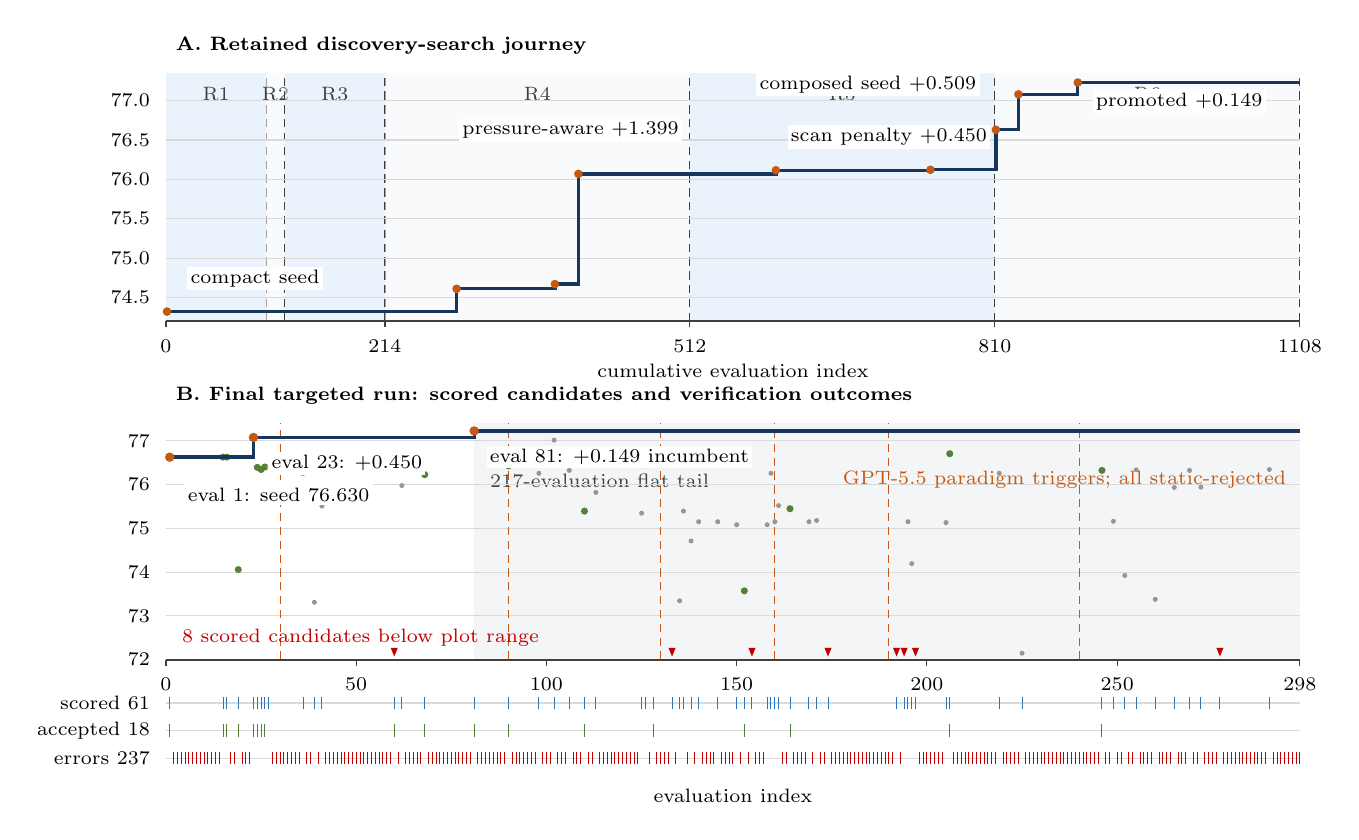
\begin{tikzpicture}[x=1cm,y=1cm]
\node[anchor=west, font=\bfseries\scriptsize] at (1.550,9.700) {A. Retained discovery-search journey};
\fill[lightblue, opacity=0.55] (1.550,6.200) rectangle (2.824,9.350);
\draw[darkgray, densely dashed] (2.824,6.200) -- (2.824,9.350);
\node[font=\scriptsize, anchor=north, text=darkgray] at (2.187,9.300) {R1};
\fill[graybg, opacity=0.55] (2.824,6.200) rectangle (3.058,9.350);
\draw[darkgray, densely dashed] (3.058,6.200) -- (3.058,9.350);
\node[font=\scriptsize, anchor=north, text=darkgray] at (2.941,9.300) {R2};
\fill[lightblue, opacity=0.55] (3.058,6.200) rectangle (4.331,9.350);
\draw[darkgray, densely dashed] (4.331,6.200) -- (4.331,9.350);
\node[font=\scriptsize, anchor=north, text=darkgray] at (3.694,9.300) {R3};
\fill[graybg, opacity=0.55] (4.331,6.200) rectangle (8.204,9.350);
\draw[darkgray, densely dashed] (8.204,6.200) -- (8.204,9.350);
\node[font=\scriptsize, anchor=north, text=darkgray] at (6.268,9.300) {R4};
\fill[lightblue, opacity=0.55] (8.204,6.200) rectangle (12.077,9.350);
\draw[darkgray, densely dashed] (12.077,6.200) -- (12.077,9.350);
\node[font=\scriptsize, anchor=north, text=darkgray] at (10.141,9.300) {R5};
\fill[graybg, opacity=0.55] (12.077,6.200) rectangle (15.950,9.350);
\draw[darkgray, densely dashed] (15.950,6.200) -- (15.950,9.350);
\node[font=\scriptsize, anchor=north, text=darkgray] at (14.014,9.300) {R6};
\draw[darkgray!20] (1.550,6.500) -- (15.950,6.500);
\node[font=\scriptsize, anchor=east] at (1.470,6.500) {74.5};
\draw[darkgray!20] (1.550,7.000) -- (15.950,7.000);
\node[font=\scriptsize, anchor=east] at (1.470,7.000) {75.0};
\draw[darkgray!20] (1.550,7.500) -- (15.950,7.500);
\node[font=\scriptsize, anchor=east] at (1.470,7.500) {75.5};
\draw[darkgray!20] (1.550,8.000) -- (15.950,8.000);
\node[font=\scriptsize, anchor=east] at (1.470,8.000) {76.0};
\draw[darkgray!20] (1.550,8.500) -- (15.950,8.500);
\node[font=\scriptsize, anchor=east] at (1.470,8.500) {76.5};
\draw[darkgray!20] (1.550,9.000) -- (15.950,9.000);
\node[font=\scriptsize, anchor=east] at (1.470,9.000) {77.0};
\draw[very thick, draw=navy] (1.563,6.321) -- (5.241,6.321) -- (5.241,6.610) -- (6.489,6.610) -- (6.489,6.670) -- (6.788,6.670) -- (6.788,8.069) -- (9.296,8.069) -- (9.296,8.115) -- (11.258,8.115) -- (11.258,8.121) -- (12.090,8.121) -- (12.090,8.630) -- (12.376,8.630) -- (12.376,9.080) -- (13.130,9.080) -- (13.130,9.230) -- (15.950,9.230);
\fill[orange] (1.563,6.321) circle (0.055);
\fill[orange] (5.241,6.610) circle (0.055);
\fill[orange] (6.489,6.670) circle (0.055);
\fill[orange] (6.788,8.069) circle (0.055);
\fill[orange] (9.296,8.115) circle (0.055);
\fill[orange] (11.258,8.121) circle (0.055);
\fill[orange] (12.090,8.630) circle (0.055);
\fill[orange] (12.376,9.080) circle (0.055);
\fill[orange] (13.130,9.230) circle (0.055);
\node[font=\scriptsize, anchor=west, fill=white, inner sep=1.2pt] at (1.813,6.741) {compact seed};
\node[font=\scriptsize, anchor=south, fill=white, inner sep=1.2pt] at (6.688,8.469) {pressure-aware +1.399};
\node[font=\scriptsize, anchor=south east, fill=white, inner sep=1.2pt] at (11.890,9.050) {composed seed +0.509};
\node[font=\scriptsize, anchor=north east, fill=white, inner sep=1.2pt] at (12.026,8.700) {scan penalty +0.450};
\node[font=\scriptsize, anchor=north west, fill=white, inner sep=1.2pt] at (13.310,9.150) {promoted +0.149};
\draw[darkgray] (1.550,6.200) -- (1.550,6.120);
\node[font=\scriptsize, anchor=north] at (1.550,6.090) {0};
\draw[darkgray] (4.331,6.200) -- (4.331,6.120);
\node[font=\scriptsize, anchor=north] at (4.331,6.090) {214};
\draw[darkgray] (8.204,6.200) -- (8.204,6.120);
\node[font=\scriptsize, anchor=north] at (8.204,6.090) {512};
\draw[darkgray] (12.077,6.200) -- (12.077,6.120);
\node[font=\scriptsize, anchor=north] at (12.077,6.090) {810};
\draw[darkgray] (15.950,6.200) -- (15.950,6.120);
\node[font=\scriptsize, anchor=north] at (15.950,6.090) {1108};
\draw[darkgray, thick] (1.550,6.200) -- (15.950,6.200);
\node[font=\scriptsize, anchor=north] at (8.750,5.780) {cumulative evaluation index};
\node[anchor=west, font=\bfseries\scriptsize] at (1.550,5.250) {B. Final targeted run: scored candidates and verification outcomes};
\fill[graybg] (5.464,1.900) rectangle (15.950,4.900);
\node[font=\scriptsize, anchor=north west, text=darkgray] at (5.544,4.380) {217-evaluation flat tail};
\draw[darkgray!20] (1.550,1.900) -- (15.950,1.900);
\node[font=\scriptsize, anchor=east] at (1.470,1.900) {72};
\draw[darkgray!20] (1.550,2.456) -- (15.950,2.456);
\node[font=\scriptsize, anchor=east] at (1.470,2.456) {73};
\draw[darkgray!20] (1.550,3.011) -- (15.950,3.011);
\node[font=\scriptsize, anchor=east] at (1.470,3.011) {74};
\draw[darkgray!20] (1.550,3.567) -- (15.950,3.567);
\node[font=\scriptsize, anchor=east] at (1.470,3.567) {75};
\draw[darkgray!20] (1.550,4.122) -- (15.950,4.122);
\node[font=\scriptsize, anchor=east] at (1.470,4.122) {76};
\draw[darkgray!20] (1.550,4.678) -- (15.950,4.678);
\node[font=\scriptsize, anchor=east] at (1.470,4.678) {77};
\draw[orange, densely dashed] (3.000,1.900) -- (3.000,4.900);
\draw[orange, densely dashed] (5.899,1.900) -- (5.899,4.900);
\draw[orange, densely dashed] (7.832,1.900) -- (7.832,4.900);
\draw[orange, densely dashed] (9.282,1.900) -- (9.282,4.900);
\draw[orange, densely dashed] (10.731,1.900) -- (10.731,4.900);
\draw[orange, densely dashed] (13.147,1.900) -- (13.147,4.900);
\node[font=\scriptsize, anchor=north east, text=orange] at (15.900,4.420) {GPT-5.5 paradigm triggers; all static-rejected};
\fill[green] (1.598,4.472) circle (0.045);
\fill[green] (2.275,4.472) circle (0.045);
\fill[green] (2.323,4.472) circle (0.045);
\fill[green] (2.468,3.044) circle (0.045);
\fill[green] (2.661,4.722) circle (0.045);
\fill[green] (2.710,4.342) circle (0.045);
\fill[green] (2.758,4.315) circle (0.045);
\fill[green] (2.806,4.347) circle (0.045);
\fill[darkgray!55] (2.855,4.347) circle (0.032);
\fill[darkgray!55] (3.290,4.264) circle (0.032);
\fill[darkgray!55] (3.435,2.629) circle (0.032);
\fill[darkgray!55] (3.531,3.851) circle (0.032);
\fill[red] (4.449,1.940) -- (4.404,2.050) -- (4.494,2.050) -- cycle;
\fill[darkgray!55] (4.546,4.111) circle (0.032);
\fill[green] (4.836,4.250) circle (0.045);
\fill[green] (5.464,4.805) circle (0.045);
\fill[green] (5.899,4.361) circle (0.045);
\fill[darkgray!55] (6.286,4.267) circle (0.032);
\fill[darkgray!55] (6.479,4.688) circle (0.032);
\fill[darkgray!55] (6.672,4.304) circle (0.032);
\fill[green] (6.865,3.787) circle (0.045);
\fill[darkgray!55] (7.010,4.024) circle (0.032);
\fill[darkgray!55] (7.590,3.760) circle (0.032);
\fill[darkgray!55] (7.639,4.361) circle (0.032);
\fill[green] (7.735,4.516) circle (0.045);
\fill[red] (7.977,1.940) -- (7.932,2.050) -- (8.022,2.050) -- cycle;
\fill[darkgray!55] (8.073,2.648) circle (0.032);
\fill[darkgray!55] (8.122,3.787) circle (0.032);
\fill[darkgray!55] (8.218,3.408) circle (0.032);
\fill[darkgray!55] (8.315,3.652) circle (0.032);
\fill[darkgray!55] (8.557,3.652) circle (0.032);
\fill[darkgray!55] (8.798,3.614) circle (0.032);
\fill[green] (8.895,2.774) circle (0.045);
\fill[red] (8.992,1.940) -- (8.947,2.050) -- (9.037,2.050) -- cycle;
\fill[darkgray!55] (9.185,3.614) circle (0.032);
\fill[darkgray!55] (9.233,4.267) circle (0.032);
\fill[darkgray!55] (9.282,3.652) circle (0.032);
\fill[darkgray!55] (9.330,3.857) circle (0.032);
\fill[green] (9.475,3.817) circle (0.045);
\fill[darkgray!55] (9.716,3.652) circle (0.032);
\fill[darkgray!55] (9.813,3.668) circle (0.032);
\fill[red] (9.958,1.940) -- (9.913,2.050) -- (10.003,2.050) -- cycle;
\fill[red] (10.828,1.940) -- (10.783,2.050) -- (10.873,2.050) -- cycle;
\fill[red] (10.924,1.940) -- (10.879,2.050) -- (10.969,2.050) -- cycle;
\fill[darkgray!55] (10.973,3.652) circle (0.032);
\fill[darkgray!55] (11.021,3.120) circle (0.032);
\fill[red] (11.069,1.940) -- (11.024,2.050) -- (11.114,2.050) -- cycle;
\fill[darkgray!55] (11.456,3.641) circle (0.032);
\fill[green] (11.504,4.516) circle (0.045);
\fill[darkgray!55] (12.133,4.267) circle (0.032);
\fill[darkgray!55] (12.422,1.982) circle (0.032);
\fill[green] (13.437,4.304) circle (0.045);
\fill[darkgray!55] (13.582,3.657) circle (0.032);
\fill[darkgray!55] (13.727,2.969) circle (0.032);
\fill[darkgray!55] (13.872,4.310) circle (0.032);
\fill[darkgray!55] (14.114,2.666) circle (0.032);
\fill[darkgray!55] (14.355,4.087) circle (0.032);
\fill[darkgray!55] (14.549,4.304) circle (0.032);
\fill[darkgray!55] (14.694,4.091) circle (0.032);
\fill[red] (14.935,1.940) -- (14.890,2.050) -- (14.980,2.050) -- cycle;
\fill[darkgray!55] (15.563,4.315) circle (0.032);
\draw[very thick, draw=navy] (1.598,4.472) -- (2.661,4.472) -- (2.661,4.722) -- (5.464,4.722) -- (5.464,4.805) -- (15.950,4.805);
\fill[orange] (1.598,4.472) circle (0.06);
\fill[orange] (2.661,4.722) circle (0.06);
\fill[orange] (5.464,4.805) circle (0.06);
\node[font=\scriptsize, anchor=north west, fill=white, inner sep=1.2pt] at (1.778,4.132) {eval 1: seed 76.630};
\node[font=\scriptsize, anchor=north west, fill=white, inner sep=1.2pt] at (2.841,4.542) {eval 23: +0.450};
\node[font=\scriptsize, anchor=north west, fill=white, inner sep=1.2pt] at (5.614,4.625) {eval 81: +0.149 incumbent};
\node[font=\scriptsize, anchor=south west, text=red] at (1.630,1.950) {8 scored candidates below plot range};
\node[font=\scriptsize, anchor=east] at (1.470,1.350) {scored 61};
\draw[darkgray!20] (1.550,1.350) -- (15.950,1.350);
\draw[blue, line width=0.35pt] (1.598,1.270) -- (1.598,1.430);
\draw[blue, line width=0.35pt] (2.275,1.270) -- (2.275,1.430);
\draw[blue, line width=0.35pt] (2.323,1.270) -- (2.323,1.430);
\draw[blue, line width=0.35pt] (2.468,1.270) -- (2.468,1.430);
\draw[blue, line width=0.35pt] (2.661,1.270) -- (2.661,1.430);
\draw[blue, line width=0.35pt] (2.710,1.270) -- (2.710,1.430);
\draw[blue, line width=0.35pt] (2.758,1.270) -- (2.758,1.430);
\draw[blue, line width=0.35pt] (2.806,1.270) -- (2.806,1.430);
\draw[blue, line width=0.35pt] (2.855,1.270) -- (2.855,1.430);
\draw[blue, line width=0.35pt] (3.290,1.270) -- (3.290,1.430);
\draw[blue, line width=0.35pt] (3.435,1.270) -- (3.435,1.430);
\draw[blue, line width=0.35pt] (3.531,1.270) -- (3.531,1.430);
\draw[blue, line width=0.35pt] (4.449,1.270) -- (4.449,1.430);
\draw[blue, line width=0.35pt] (4.546,1.270) -- (4.546,1.430);
\draw[blue, line width=0.35pt] (4.836,1.270) -- (4.836,1.430);
\draw[blue, line width=0.35pt] (5.464,1.270) -- (5.464,1.430);
\draw[blue, line width=0.35pt] (5.899,1.270) -- (5.899,1.430);
\draw[blue, line width=0.35pt] (6.286,1.270) -- (6.286,1.430);
\draw[blue, line width=0.35pt] (6.479,1.270) -- (6.479,1.430);
\draw[blue, line width=0.35pt] (6.672,1.270) -- (6.672,1.430);
\draw[blue, line width=0.35pt] (6.865,1.270) -- (6.865,1.430);
\draw[blue, line width=0.35pt] (7.010,1.270) -- (7.010,1.430);
\draw[blue, line width=0.35pt] (7.590,1.270) -- (7.590,1.430);
\draw[blue, line width=0.35pt] (7.639,1.270) -- (7.639,1.430);
\draw[blue, line width=0.35pt] (7.735,1.270) -- (7.735,1.430);
\draw[blue, line width=0.35pt] (7.977,1.270) -- (7.977,1.430);
\draw[blue, line width=0.35pt] (8.073,1.270) -- (8.073,1.430);
\draw[blue, line width=0.35pt] (8.122,1.270) -- (8.122,1.430);
\draw[blue, line width=0.35pt] (8.218,1.270) -- (8.218,1.430);
\draw[blue, line width=0.35pt] (8.315,1.270) -- (8.315,1.430);
\draw[blue, line width=0.35pt] (8.557,1.270) -- (8.557,1.430);
\draw[blue, line width=0.35pt] (8.798,1.270) -- (8.798,1.430);
\draw[blue, line width=0.35pt] (8.895,1.270) -- (8.895,1.430);
\draw[blue, line width=0.35pt] (8.992,1.270) -- (8.992,1.430);
\draw[blue, line width=0.35pt] (9.185,1.270) -- (9.185,1.430);
\draw[blue, line width=0.35pt] (9.233,1.270) -- (9.233,1.430);
\draw[blue, line width=0.35pt] (9.282,1.270) -- (9.282,1.430);
\draw[blue, line width=0.35pt] (9.330,1.270) -- (9.330,1.430);
\draw[blue, line width=0.35pt] (9.475,1.270) -- (9.475,1.430);
\draw[blue, line width=0.35pt] (9.716,1.270) -- (9.716,1.430);
\draw[blue, line width=0.35pt] (9.813,1.270) -- (9.813,1.430);
\draw[blue, line width=0.35pt] (9.958,1.270) -- (9.958,1.430);
\draw[blue, line width=0.35pt] (10.828,1.270) -- (10.828,1.430);
\draw[blue, line width=0.35pt] (10.924,1.270) -- (10.924,1.430);
\draw[blue, line width=0.35pt] (10.973,1.270) -- (10.973,1.430);
\draw[blue, line width=0.35pt] (11.021,1.270) -- (11.021,1.430);
\draw[blue, line width=0.35pt] (11.069,1.270) -- (11.069,1.430);
\draw[blue, line width=0.35pt] (11.456,1.270) -- (11.456,1.430);
\draw[blue, line width=0.35pt] (11.504,1.270) -- (11.504,1.430);
\draw[blue, line width=0.35pt] (12.133,1.270) -- (12.133,1.430);
\draw[blue, line width=0.35pt] (12.422,1.270) -- (12.422,1.430);
\draw[blue, line width=0.35pt] (13.437,1.270) -- (13.437,1.430);
\draw[blue, line width=0.35pt] (13.582,1.270) -- (13.582,1.430);
\draw[blue, line width=0.35pt] (13.727,1.270) -- (13.727,1.430);
\draw[blue, line width=0.35pt] (13.872,1.270) -- (13.872,1.430);
\draw[blue, line width=0.35pt] (14.114,1.270) -- (14.114,1.430);
\draw[blue, line width=0.35pt] (14.355,1.270) -- (14.355,1.430);
\draw[blue, line width=0.35pt] (14.549,1.270) -- (14.549,1.430);
\draw[blue, line width=0.35pt] (14.694,1.270) -- (14.694,1.430);
\draw[blue, line width=0.35pt] (14.935,1.270) -- (14.935,1.430);
\draw[blue, line width=0.35pt] (15.563,1.270) -- (15.563,1.430);
\node[font=\scriptsize, anchor=east] at (1.470,1.000) {accepted 18};
\draw[darkgray!20] (1.550,1.000) -- (15.950,1.000);
\draw[green, line width=0.35pt] (1.598,0.920) -- (1.598,1.080);
\draw[green, line width=0.35pt] (2.275,0.920) -- (2.275,1.080);
\draw[green, line width=0.35pt] (2.323,0.920) -- (2.323,1.080);
\draw[green, line width=0.35pt] (2.468,0.920) -- (2.468,1.080);
\draw[green, line width=0.35pt] (2.661,0.920) -- (2.661,1.080);
\draw[green, line width=0.35pt] (2.710,0.920) -- (2.710,1.080);
\draw[green, line width=0.35pt] (2.758,0.920) -- (2.758,1.080);
\draw[green, line width=0.35pt] (2.806,0.920) -- (2.806,1.080);
\draw[green, line width=0.35pt] (4.449,0.920) -- (4.449,1.080);
\draw[green, line width=0.35pt] (4.836,0.920) -- (4.836,1.080);
\draw[green, line width=0.35pt] (5.464,0.920) -- (5.464,1.080);
\draw[green, line width=0.35pt] (5.899,0.920) -- (5.899,1.080);
\draw[green, line width=0.35pt] (6.865,0.920) -- (6.865,1.080);
\draw[green, line width=0.35pt] (7.735,0.920) -- (7.735,1.080);
\draw[green, line width=0.35pt] (8.895,0.920) -- (8.895,1.080);
\draw[green, line width=0.35pt] (9.475,0.920) -- (9.475,1.080);
\draw[green, line width=0.35pt] (11.504,0.920) -- (11.504,1.080);
\draw[green, line width=0.35pt] (13.437,0.920) -- (13.437,1.080);
\node[font=\scriptsize, anchor=east] at (1.470,0.650) {errors 237};
\draw[darkgray!20] (1.550,0.650) -- (15.950,0.650);
\draw[red, line width=0.35pt] (1.647,0.570) -- (1.647,0.730);
\draw[red, line width=0.35pt] (1.695,0.570) -- (1.695,0.730);
\draw[red, line width=0.35pt] (1.743,0.570) -- (1.743,0.730);
\draw[red, line width=0.35pt] (1.792,0.570) -- (1.792,0.730);
\draw[red, line width=0.35pt] (1.840,0.570) -- (1.840,0.730);
\draw[red, line width=0.35pt] (1.888,0.570) -- (1.888,0.730);
\draw[red, line width=0.35pt] (1.937,0.570) -- (1.937,0.730);
\draw[red, line width=0.35pt] (1.985,0.570) -- (1.985,0.730);
\draw[red, line width=0.35pt] (2.033,0.570) -- (2.033,0.730);
\draw[red, line width=0.35pt] (2.082,0.570) -- (2.082,0.730);
\draw[red, line width=0.35pt] (2.130,0.570) -- (2.130,0.730);
\draw[red, line width=0.35pt] (2.178,0.570) -- (2.178,0.730);
\draw[red, line width=0.35pt] (2.227,0.570) -- (2.227,0.730);
\draw[red, line width=0.35pt] (2.371,0.570) -- (2.371,0.730);
\draw[red, line width=0.35pt] (2.420,0.570) -- (2.420,0.730);
\draw[red, line width=0.35pt] (2.516,0.570) -- (2.516,0.730);
\draw[red, line width=0.35pt] (2.565,0.570) -- (2.565,0.730);
\draw[red, line width=0.35pt] (2.613,0.570) -- (2.613,0.730);
\draw[red, line width=0.35pt] (2.903,0.570) -- (2.903,0.730);
\draw[red, line width=0.35pt] (2.951,0.570) -- (2.951,0.730);
\draw[red, line width=0.35pt] (3.000,0.570) -- (3.000,0.730);
\draw[red, line width=0.35pt] (3.048,0.570) -- (3.048,0.730);
\draw[red, line width=0.35pt] (3.096,0.570) -- (3.096,0.730);
\draw[red, line width=0.35pt] (3.145,0.570) -- (3.145,0.730);
\draw[red, line width=0.35pt] (3.193,0.570) -- (3.193,0.730);
\draw[red, line width=0.35pt] (3.241,0.570) -- (3.241,0.730);
\draw[red, line width=0.35pt] (3.338,0.570) -- (3.338,0.730);
\draw[red, line width=0.35pt] (3.386,0.570) -- (3.386,0.730);
\draw[red, line width=0.35pt] (3.483,0.570) -- (3.483,0.730);
\draw[red, line width=0.35pt] (3.580,0.570) -- (3.580,0.730);
\draw[red, line width=0.35pt] (3.628,0.570) -- (3.628,0.730);
\draw[red, line width=0.35pt] (3.676,0.570) -- (3.676,0.730);
\draw[red, line width=0.35pt] (3.724,0.570) -- (3.724,0.730);
\draw[red, line width=0.35pt] (3.773,0.570) -- (3.773,0.730);
\draw[red, line width=0.35pt] (3.821,0.570) -- (3.821,0.730);
\draw[red, line width=0.35pt] (3.869,0.570) -- (3.869,0.730);
\draw[red, line width=0.35pt] (3.918,0.570) -- (3.918,0.730);
\draw[red, line width=0.35pt] (3.966,0.570) -- (3.966,0.730);
\draw[red, line width=0.35pt] (4.014,0.570) -- (4.014,0.730);
\draw[red, line width=0.35pt] (4.063,0.570) -- (4.063,0.730);
\draw[red, line width=0.35pt] (4.111,0.570) -- (4.111,0.730);
\draw[red, line width=0.35pt] (4.159,0.570) -- (4.159,0.730);
\draw[red, line width=0.35pt] (4.208,0.570) -- (4.208,0.730);
\draw[red, line width=0.35pt] (4.256,0.570) -- (4.256,0.730);
\draw[red, line width=0.35pt] (4.304,0.570) -- (4.304,0.730);
\draw[red, line width=0.35pt] (4.353,0.570) -- (4.353,0.730);
\draw[red, line width=0.35pt] (4.401,0.570) -- (4.401,0.730);
\draw[red, line width=0.35pt] (4.498,0.570) -- (4.498,0.730);
\draw[red, line width=0.35pt] (4.594,0.570) -- (4.594,0.730);
\draw[red, line width=0.35pt] (4.643,0.570) -- (4.643,0.730);
\draw[red, line width=0.35pt] (4.691,0.570) -- (4.691,0.730);
\draw[red, line width=0.35pt] (4.739,0.570) -- (4.739,0.730);
\draw[red, line width=0.35pt] (4.788,0.570) -- (4.788,0.730);
\draw[red, line width=0.35pt] (4.884,0.570) -- (4.884,0.730);
\draw[red, line width=0.35pt] (4.933,0.570) -- (4.933,0.730);
\draw[red, line width=0.35pt] (4.981,0.570) -- (4.981,0.730);
\draw[red, line width=0.35pt] (5.029,0.570) -- (5.029,0.730);
\draw[red, line width=0.35pt] (5.078,0.570) -- (5.078,0.730);
\draw[red, line width=0.35pt] (5.126,0.570) -- (5.126,0.730);
\draw[red, line width=0.35pt] (5.174,0.570) -- (5.174,0.730);
\draw[red, line width=0.35pt] (5.222,0.570) -- (5.222,0.730);
\draw[red, line width=0.35pt] (5.271,0.570) -- (5.271,0.730);
\draw[red, line width=0.35pt] (5.319,0.570) -- (5.319,0.730);
\draw[red, line width=0.35pt] (5.367,0.570) -- (5.367,0.730);
\draw[red, line width=0.35pt] (5.416,0.570) -- (5.416,0.730);
\draw[red, line width=0.35pt] (5.512,0.570) -- (5.512,0.730);
\draw[red, line width=0.35pt] (5.561,0.570) -- (5.561,0.730);
\draw[red, line width=0.35pt] (5.609,0.570) -- (5.609,0.730);
\draw[red, line width=0.35pt] (5.657,0.570) -- (5.657,0.730);
\draw[red, line width=0.35pt] (5.706,0.570) -- (5.706,0.730);
\draw[red, line width=0.35pt] (5.754,0.570) -- (5.754,0.730);
\draw[red, line width=0.35pt] (5.802,0.570) -- (5.802,0.730);
\draw[red, line width=0.35pt] (5.851,0.570) -- (5.851,0.730);
\draw[red, line width=0.35pt] (5.947,0.570) -- (5.947,0.730);
\draw[red, line width=0.35pt] (5.996,0.570) -- (5.996,0.730);
\draw[red, line width=0.35pt] (6.044,0.570) -- (6.044,0.730);
\draw[red, line width=0.35pt] (6.092,0.570) -- (6.092,0.730);
\draw[red, line width=0.35pt] (6.141,0.570) -- (6.141,0.730);
\draw[red, line width=0.35pt] (6.189,0.570) -- (6.189,0.730);
\draw[red, line width=0.35pt] (6.237,0.570) -- (6.237,0.730);
\draw[red, line width=0.35pt] (6.334,0.570) -- (6.334,0.730);
\draw[red, line width=0.35pt] (6.382,0.570) -- (6.382,0.730);
\draw[red, line width=0.35pt] (6.431,0.570) -- (6.431,0.730);
\draw[red, line width=0.35pt] (6.527,0.570) -- (6.527,0.730);
\draw[red, line width=0.35pt] (6.576,0.570) -- (6.576,0.730);
\draw[red, line width=0.35pt] (6.624,0.570) -- (6.624,0.730);
\draw[red, line width=0.35pt] (6.720,0.570) -- (6.720,0.730);
\draw[red, line width=0.35pt] (6.769,0.570) -- (6.769,0.730);
\draw[red, line width=0.35pt] (6.817,0.570) -- (6.817,0.730);
\draw[red, line width=0.35pt] (6.914,0.570) -- (6.914,0.730);
\draw[red, line width=0.35pt] (6.962,0.570) -- (6.962,0.730);
\draw[red, line width=0.35pt] (7.059,0.570) -- (7.059,0.730);
\draw[red, line width=0.35pt] (7.107,0.570) -- (7.107,0.730);
\draw[red, line width=0.35pt] (7.155,0.570) -- (7.155,0.730);
\draw[red, line width=0.35pt] (7.204,0.570) -- (7.204,0.730);
\draw[red, line width=0.35pt] (7.252,0.570) -- (7.252,0.730);
\draw[red, line width=0.35pt] (7.300,0.570) -- (7.300,0.730);
\draw[red, line width=0.35pt] (7.349,0.570) -- (7.349,0.730);
\draw[red, line width=0.35pt] (7.397,0.570) -- (7.397,0.730);
\draw[red, line width=0.35pt] (7.445,0.570) -- (7.445,0.730);
\draw[red, line width=0.35pt] (7.494,0.570) -- (7.494,0.730);
\draw[red, line width=0.35pt] (7.542,0.570) -- (7.542,0.730);
\draw[red, line width=0.35pt] (7.687,0.570) -- (7.687,0.730);
\draw[red, line width=0.35pt] (7.784,0.570) -- (7.784,0.730);
\draw[red, line width=0.35pt] (7.832,0.570) -- (7.832,0.730);
\draw[red, line width=0.35pt] (7.880,0.570) -- (7.880,0.730);
\draw[red, line width=0.35pt] (7.929,0.570) -- (7.929,0.730);
\draw[red, line width=0.35pt] (8.025,0.570) -- (8.025,0.730);
\draw[red, line width=0.35pt] (8.170,0.570) -- (8.170,0.730);
\draw[red, line width=0.35pt] (8.267,0.570) -- (8.267,0.730);
\draw[red, line width=0.35pt] (8.363,0.570) -- (8.363,0.730);
\draw[red, line width=0.35pt] (8.412,0.570) -- (8.412,0.730);
\draw[red, line width=0.35pt] (8.460,0.570) -- (8.460,0.730);
\draw[red, line width=0.35pt] (8.508,0.570) -- (8.508,0.730);
\draw[red, line width=0.35pt] (8.605,0.570) -- (8.605,0.730);
\draw[red, line width=0.35pt] (8.653,0.570) -- (8.653,0.730);
\draw[red, line width=0.35pt] (8.702,0.570) -- (8.702,0.730);
\draw[red, line width=0.35pt] (8.750,0.570) -- (8.750,0.730);
\draw[red, line width=0.35pt] (8.847,0.570) -- (8.847,0.730);
\draw[red, line width=0.35pt] (8.943,0.570) -- (8.943,0.730);
\draw[red, line width=0.35pt] (9.040,0.570) -- (9.040,0.730);
\draw[red, line width=0.35pt] (9.088,0.570) -- (9.088,0.730);
\draw[red, line width=0.35pt] (9.137,0.570) -- (9.137,0.730);
\draw[red, line width=0.35pt] (9.378,0.570) -- (9.378,0.730);
\draw[red, line width=0.35pt] (9.427,0.570) -- (9.427,0.730);
\draw[red, line width=0.35pt] (9.523,0.570) -- (9.523,0.730);
\draw[red, line width=0.35pt] (9.571,0.570) -- (9.571,0.730);
\draw[red, line width=0.35pt] (9.620,0.570) -- (9.620,0.730);
\draw[red, line width=0.35pt] (9.668,0.570) -- (9.668,0.730);
\draw[red, line width=0.35pt] (9.765,0.570) -- (9.765,0.730);
\draw[red, line width=0.35pt] (9.861,0.570) -- (9.861,0.730);
\draw[red, line width=0.35pt] (9.910,0.570) -- (9.910,0.730);
\draw[red, line width=0.35pt] (10.006,0.570) -- (10.006,0.730);
\draw[red, line width=0.35pt] (10.055,0.570) -- (10.055,0.730);
\draw[red, line width=0.35pt] (10.103,0.570) -- (10.103,0.730);
\draw[red, line width=0.35pt] (10.151,0.570) -- (10.151,0.730);
\draw[red, line width=0.35pt] (10.200,0.570) -- (10.200,0.730);
\draw[red, line width=0.35pt] (10.248,0.570) -- (10.248,0.730);
\draw[red, line width=0.35pt] (10.296,0.570) -- (10.296,0.730);
\draw[red, line width=0.35pt] (10.345,0.570) -- (10.345,0.730);
\draw[red, line width=0.35pt] (10.393,0.570) -- (10.393,0.730);
\draw[red, line width=0.35pt] (10.441,0.570) -- (10.441,0.730);
\draw[red, line width=0.35pt] (10.490,0.570) -- (10.490,0.730);
\draw[red, line width=0.35pt] (10.538,0.570) -- (10.538,0.730);
\draw[red, line width=0.35pt] (10.586,0.570) -- (10.586,0.730);
\draw[red, line width=0.35pt] (10.635,0.570) -- (10.635,0.730);
\draw[red, line width=0.35pt] (10.683,0.570) -- (10.683,0.730);
\draw[red, line width=0.35pt] (10.731,0.570) -- (10.731,0.730);
\draw[red, line width=0.35pt] (10.780,0.570) -- (10.780,0.730);
\draw[red, line width=0.35pt] (10.876,0.570) -- (10.876,0.730);
\draw[red, line width=0.35pt] (11.118,0.570) -- (11.118,0.730);
\draw[red, line width=0.35pt] (11.166,0.570) -- (11.166,0.730);
\draw[red, line width=0.35pt] (11.214,0.570) -- (11.214,0.730);
\draw[red, line width=0.35pt] (11.263,0.570) -- (11.263,0.730);
\draw[red, line width=0.35pt] (11.311,0.570) -- (11.311,0.730);
\draw[red, line width=0.35pt] (11.359,0.570) -- (11.359,0.730);
\draw[red, line width=0.35pt] (11.408,0.570) -- (11.408,0.730);
\draw[red, line width=0.35pt] (11.553,0.570) -- (11.553,0.730);
\draw[red, line width=0.35pt] (11.601,0.570) -- (11.601,0.730);
\draw[red, line width=0.35pt] (11.649,0.570) -- (11.649,0.730);
\draw[red, line width=0.35pt] (11.698,0.570) -- (11.698,0.730);
\draw[red, line width=0.35pt] (11.746,0.570) -- (11.746,0.730);
\draw[red, line width=0.35pt] (11.794,0.570) -- (11.794,0.730);
\draw[red, line width=0.35pt] (11.843,0.570) -- (11.843,0.730);
\draw[red, line width=0.35pt] (11.891,0.570) -- (11.891,0.730);
\draw[red, line width=0.35pt] (11.939,0.570) -- (11.939,0.730);
\draw[red, line width=0.35pt] (11.988,0.570) -- (11.988,0.730);
\draw[red, line width=0.35pt] (12.036,0.570) -- (12.036,0.730);
\draw[red, line width=0.35pt] (12.084,0.570) -- (12.084,0.730);
\draw[red, line width=0.35pt] (12.181,0.570) -- (12.181,0.730);
\draw[red, line width=0.35pt] (12.229,0.570) -- (12.229,0.730);
\draw[red, line width=0.35pt] (12.278,0.570) -- (12.278,0.730);
\draw[red, line width=0.35pt] (12.326,0.570) -- (12.326,0.730);
\draw[red, line width=0.35pt] (12.374,0.570) -- (12.374,0.730);
\draw[red, line width=0.35pt] (12.471,0.570) -- (12.471,0.730);
\draw[red, line width=0.35pt] (12.519,0.570) -- (12.519,0.730);
\draw[red, line width=0.35pt] (12.567,0.570) -- (12.567,0.730);
\draw[red, line width=0.35pt] (12.616,0.570) -- (12.616,0.730);
\draw[red, line width=0.35pt] (12.664,0.570) -- (12.664,0.730);
\draw[red, line width=0.35pt] (12.712,0.570) -- (12.712,0.730);
\draw[red, line width=0.35pt] (12.761,0.570) -- (12.761,0.730);
\draw[red, line width=0.35pt] (12.809,0.570) -- (12.809,0.730);
\draw[red, line width=0.35pt] (12.857,0.570) -- (12.857,0.730);
\draw[red, line width=0.35pt] (12.906,0.570) -- (12.906,0.730);
\draw[red, line width=0.35pt] (12.954,0.570) -- (12.954,0.730);
\draw[red, line width=0.35pt] (13.002,0.570) -- (13.002,0.730);
\draw[red, line width=0.35pt] (13.051,0.570) -- (13.051,0.730);
\draw[red, line width=0.35pt] (13.099,0.570) -- (13.099,0.730);
\draw[red, line width=0.35pt] (13.147,0.570) -- (13.147,0.730);
\draw[red, line width=0.35pt] (13.196,0.570) -- (13.196,0.730);
\draw[red, line width=0.35pt] (13.244,0.570) -- (13.244,0.730);
\draw[red, line width=0.35pt] (13.292,0.570) -- (13.292,0.730);
\draw[red, line width=0.35pt] (13.341,0.570) -- (13.341,0.730);
\draw[red, line width=0.35pt] (13.389,0.570) -- (13.389,0.730);
\draw[red, line width=0.35pt] (13.486,0.570) -- (13.486,0.730);
\draw[red, line width=0.35pt] (13.534,0.570) -- (13.534,0.730);
\draw[red, line width=0.35pt] (13.631,0.570) -- (13.631,0.730);
\draw[red, line width=0.35pt] (13.679,0.570) -- (13.679,0.730);
\draw[red, line width=0.35pt] (13.776,0.570) -- (13.776,0.730);
\draw[red, line width=0.35pt] (13.824,0.570) -- (13.824,0.730);
\draw[red, line width=0.35pt] (13.920,0.570) -- (13.920,0.730);
\draw[red, line width=0.35pt] (13.969,0.570) -- (13.969,0.730);
\draw[red, line width=0.35pt] (14.017,0.570) -- (14.017,0.730);
\draw[red, line width=0.35pt] (14.065,0.570) -- (14.065,0.730);
\draw[red, line width=0.35pt] (14.162,0.570) -- (14.162,0.730);
\draw[red, line width=0.35pt] (14.210,0.570) -- (14.210,0.730);
\draw[red, line width=0.35pt] (14.259,0.570) -- (14.259,0.730);
\draw[red, line width=0.35pt] (14.307,0.570) -- (14.307,0.730);
\draw[red, line width=0.35pt] (14.404,0.570) -- (14.404,0.730);
\draw[red, line width=0.35pt] (14.452,0.570) -- (14.452,0.730);
\draw[red, line width=0.35pt] (14.500,0.570) -- (14.500,0.730);
\draw[red, line width=0.35pt] (14.597,0.570) -- (14.597,0.730);
\draw[red, line width=0.35pt] (14.645,0.570) -- (14.645,0.730);
\draw[red, line width=0.35pt] (14.742,0.570) -- (14.742,0.730);
\draw[red, line width=0.35pt] (14.790,0.570) -- (14.790,0.730);
\draw[red, line width=0.35pt] (14.839,0.570) -- (14.839,0.730);
\draw[red, line width=0.35pt] (14.887,0.570) -- (14.887,0.730);
\draw[red, line width=0.35pt] (14.984,0.570) -- (14.984,0.730);
\draw[red, line width=0.35pt] (15.032,0.570) -- (15.032,0.730);
\draw[red, line width=0.35pt] (15.080,0.570) -- (15.080,0.730);
\draw[red, line width=0.35pt] (15.129,0.570) -- (15.129,0.730);
\draw[red, line width=0.35pt] (15.177,0.570) -- (15.177,0.730);
\draw[red, line width=0.35pt] (15.225,0.570) -- (15.225,0.730);
\draw[red, line width=0.35pt] (15.273,0.570) -- (15.273,0.730);
\draw[red, line width=0.35pt] (15.322,0.570) -- (15.322,0.730);
\draw[red, line width=0.35pt] (15.370,0.570) -- (15.370,0.730);
\draw[red, line width=0.35pt] (15.418,0.570) -- (15.418,0.730);
\draw[red, line width=0.35pt] (15.467,0.570) -- (15.467,0.730);
\draw[red, line width=0.35pt] (15.515,0.570) -- (15.515,0.730);
\draw[red, line width=0.35pt] (15.612,0.570) -- (15.612,0.730);
\draw[red, line width=0.35pt] (15.660,0.570) -- (15.660,0.730);
\draw[red, line width=0.35pt] (15.708,0.570) -- (15.708,0.730);
\draw[red, line width=0.35pt] (15.757,0.570) -- (15.757,0.730);
\draw[red, line width=0.35pt] (15.805,0.570) -- (15.805,0.730);
\draw[red, line width=0.35pt] (15.853,0.570) -- (15.853,0.730);
\draw[red, line width=0.35pt] (15.902,0.570) -- (15.902,0.730);
\draw[red, line width=0.35pt] (15.950,0.570) -- (15.950,0.730);
\draw[darkgray] (1.550,1.900) -- (1.550,1.820);
\node[font=\scriptsize, anchor=north] at (1.550,1.790) {0};
\draw[darkgray] (3.966,1.900) -- (3.966,1.820);
\node[font=\scriptsize, anchor=north] at (3.966,1.790) {50};
\draw[darkgray] (6.382,1.900) -- (6.382,1.820);
\node[font=\scriptsize, anchor=north] at (6.382,1.790) {100};
\draw[darkgray] (8.798,1.900) -- (8.798,1.820);
\node[font=\scriptsize, anchor=north] at (8.798,1.790) {150};
\draw[darkgray] (11.214,1.900) -- (11.214,1.820);
\node[font=\scriptsize, anchor=north] at (11.214,1.790) {200};
\draw[darkgray] (13.631,1.900) -- (13.631,1.820);
\node[font=\scriptsize, anchor=north] at (13.631,1.790) {250};
\draw[darkgray] (15.950,1.900) -- (15.950,1.820);
\node[font=\scriptsize, anchor=north] at (15.950,1.790) {298};
\draw[darkgray, thick] (1.550,1.900) -- (15.950,1.900);
\node[font=\scriptsize, anchor=north] at (8.750,0.380) {evaluation index};
\end{tikzpicture}%
}

\caption{Evaluation trajectory leading to the promoted incumbent.  Panel A concatenates
the six retained discovery-verifier runs in Table~\ref{tab:journey-runs} and plots the
global best score, so a flat segment means that additional evaluations did not improve
the retained policy.  Panel B expands the final targeted run: gray and green points are
successfully scored candidates, green points entered or replaced an archive cell,
orange points are strict global-best jumps, red triangles are scored candidates below
the displayed score range, and the outcome raster distinguishes scored, accepted, and
failed generation or static-verification attempts.  Dashed orange lines mark
GPT-5.5 paradigm-shift triggers.}
\label{fig:incumbent-eval-trajectory}
\end{figure}

Figure~\ref{fig:incumbent-eval-trajectory} makes the search path more explicit than the
final-score table alone.  The first three retained runs consumed 214 evaluations
without improving the \(74.321\) compact seed.  In the first long compact-family run,
a normal mutation reached \(74.610\), a punctuated-equilibrium paradigm shift reached
\(74.670\), and a later normal mutation made the largest jump in the retained journey,
\(+1.399\) to the \(76.069\) pressure-aware policy.  The follow-up run added only
\(0.051\).  Manual composition of its useful persistent-pressure term with
recurrence-gated depth relief produced the \(76.630\) seed used by the final targeted
run.

Within that final run, evaluation 23 found a frequency-and-priority scan-penalty
alternative at \(77.080\).  Evaluation 81 found the promoted priority-aware pressure
hinge at \(77.230\).  The latter was not merely the end of a smooth climb: it was the
last strict improvement, and the remaining 217 evaluations did not move the global
best.  Only 61 of 298 attempted evaluations produced a score, 18 entered or replaced
an archive cell, and 237 failed generation or static verification.  All six direct
GPT-5.5 paradigm-shift candidates in this run were rejected for effective complexity
between 669 and 739, above the 650-node limit.  The figure is generated directly from
the retained Levi snapshots by
\filepath{scripts/plot_prefix_kv_eval_trajectory.py}.

The run diary shows why simply increasing the evaluation budget was not the answer.
The first 100-run generated a more complicated but worse policy.  The twenty-iteration
run confirmed plumbing, not search quality.  Another 100-run produced a plausible but
behaviorally inert edit.  The first 300-run finally found a useful pressure-aware
mechanism, but later runs exposed archive collapse and long periods with no
improvement.  The successful June 8 run did not merely spend more budget: it changed
what feedback the generator received and what specialist behavior the archive could
retain.

The successful run still documents substantial remaining friction.  It accepted 18
candidates but recorded 237 generation or static-check errors.  Its winner appeared at
evaluation 81, and the remaining 217 evaluations did not improve it.  This means the
system had become capable of finding useful compact changes, but generator compliance
and late-run marginal value were still weak.

\subsection{The structured-policy detour}

The project also took a deliberate detour through richer state representations.  The
observable surface was expanded with recurrence, subtree, and regime context, and a
bounded \code{MultiTimescaleDecay} primitive was added to make multi-timescale state
available without unbounded dictionaries.

The first expansion run showed that supplying a primitive was not enough.  The
strongest generated policy used hand-written fast and slow state, reached 1239
effective nodes, and the only archived primitive user was invalid.  The prompt and seed
were then changed to demonstrate \code{observe_vector}, and form-aware complexity gave
canonical calls a bounded credit.  All 24 archived elites across three subsequent
98-evaluation searches adopted the primitive, proving the adoption intervention
worked.

Those runs still did not produce a deployable winner.  Their strongest generated
programs had 1198--1429 effective nodes.  Manual behavior-only ablation then provided
the useful result that evolution alone had not isolated:

\begin{itemize}
  \item broad recurrence state was harmful and increased churn;
  \item priority-decay state was inert;
  \item subtree and regime context carried value;
  \item miss state was nearly neutral on validation but protected cyclic behavior.
\end{itemize}

This detour established the current division of labor.  LLM evolution is useful for
proposing structure; controlled deletion ablation identifies which pieces carry
behavior; deterministic tuning handles compact coefficients; and final adjudication
decides whether the complete source is deployable.  Expecting one search loop to do
all four jobs was inefficient.

\subsection{From the first gain to the promoted incumbent}

The first clear discovery-verifier improvement was the \(76.069\) pressure-aware policy.
It reduced churn by conditioning admission on sustained pressure rather than admitting
every plausible suffix.  A subsequent run discovered a narrow persistent-pressure
threshold term.  That term was not sufficient alone, but it was retained and composed
with recurrence-gated depth relief, producing the \(76.630\) parent used by the
retained discovery search.

The final step depended on search-process changes motivated by the earlier failures.
Every normal mutation received diagnostics for the non-quarantined
\identifier{agentic_tool_workflows} surrogate and selectable
\identifier{stochastic_serving_mix}; the archive could retain specialists for those
behaviors; and the held-out agent probe remained excluded from selection behind an
automatic divergence tripwire.  The resulting winner added one priority-aware
pressure term, raised charged selection from \(76.630\) to \(77.230\), cut validation
churn by \(37.6\%\), and improved hidden score.

Promotion still required manual-style scientific checks encoded in artifacts: exact
seed-versus-winner ablation, raw-before-complexity decomposition, aggregate probe
inspection, hidden evaluation, and the agentic tripwire.  The apparent charged probe
regression was entirely complexity accounting; raw probe behavior improved.  Without
that decomposition, the same candidate could have been rejected for the wrong reason
or promoted without adequate evidence.

\subsection{Where the journey stands}

The production full-policy lane has now crossed the 16-token TinyLFU-LRU target without
hand-authoring the candidate.  Its 300-evaluation search first found a \(656\)-node,
\(64.779\)-score exploration winner.  A separate 100-evaluation simplification phase
found a \(539\)-node top scorer at \(66.033\), but promotion correctly rejected it
because its agentic surrogate-to-probe gap was \(0.1217\), just above the \(0.12\)
limit.  The next archived elite scored \(65.649\) at \(572\) nodes and passed the same
tripwire with a \(0.0918\) gap.  It also improved the hidden score from
TinyLFU-LRU's \(-2.789\) to \(3.064\).  This result supports a two-stage search rule:
allow measured over-cap proposals to expose useful structure, then let search perform
explicit simplification and adjudicate all resulting elites rather than automatically
promoting the scalar winner.

The associated cost claim must include both stages.  The production run cost
\$4.133, and the required simplification run cost \$0.937, for a direct final-stage
total of \$5.070 across 397 evaluations.  Including the six retained
discovery-verifier runs that produced the seed and search-process changes raises the
retained lineage to \$21.981 across 1,505 evaluations.  Adding the documented
old-verifier, structured-policy, and two eviction-specialist stages yields a
pre-promotion research total of at least \$44.845 across 2,989 evaluations.  This is
still a lower bound because deterministic sweeps, local simulator compute, manual
analysis, and unretained experiments are not priced.  The auditable breakdown is
retained in \filepath{docs/results/search_cost_tally.md}.

The practical gain was therefore not one-shot cheapness.  The workflow made the
research loop faster: a failed candidate could be decomposed into behavior,
complexity, and generalization effects; a useful fragment could seed a specialist or
simplification stage; and the resulting lesson could become a falsifiable follow-up
without rebuilding the experimental harness.  That iteration velocity is a central
result of the project, while cumulative cost remains the honest accounting unit for
the promoted algorithm.

A fixed-block-count geometry sweep then tested both incumbents at 24, 48, 96, and
128 blocks.  Jointly scoring those four tiers, the new policy improves the 16-token
score from \(64.702\) to \(66.710\), but lowers the 8-token score from \(74.068\) to
\(63.154\).  At 8 tokens it reduces churn but raises avoidable-rejection regret by
roughly 3.9--6.1 percentage points and lowers validation token hit by 1.3--2.1
percentage points.  The admission threshold learned for 16-token blocks is therefore
too selective for finer-grained cache entries, especially after capacity becomes
large enough that eviction pressure subsides.  Promotion is consequently scoped to
16-token deployments; a geometry-robust successor must include both block sizes in
selection.  Full results are retained in
\filepath{docs/results/incumbent_geometry_sweep.md}.

A second sweep held cache capacity fixed at 384 and 768 tokens while increasing
physical block size through 16, 24, 32, 48, and 64 tokens.  This falsified the
simple hypothesis that the new admission policy benefits monotonically from coarser
blocks.  The new incumbent's charged scores were \(65.649\), \(3.006\),
\(-17.602\), \(-40.346\), and \(-37.107\), respectively.  Request-level p10 fell
from \(0.256\) at 16 tokens to \(0.062\) at 24 and zero at 32 tokens.  Raw scores
were already negative from 32 tokens onward, so complexity accounting is not the
cause.  Coarse blocks instead destroy reusable-prefix resolution and reduce the
number of independently retainable cache entries.  Sixteen tokens is the optimum
of the tested coarse range; further crossover work should concentrate between 8 and
24 tokens.  The complete table is retained in
\filepath{docs/results/block_granularity_sweep.md}.

A follow-up increased block capacity to 24, 48, 96, and 128 entries for every coarse
block size.  Capacity restored the 24-token aggregate hit rate to \(0.667\) and
request p10 to \(0.262\) at 128 blocks, but its joint score remained \(21.653\)
versus \(66.710\) at 16 tokens.  The fairness cost rose from \(7.749\) to \(21.996\),
and tenant-phase-shift hit fell to \(0.330\).  At 32 tokens and above, some workload
families retained exactly zero token hit irrespective of the larger capacity.  The
curves largely saturated by 96 blocks.  More entries therefore relieve pressure but
cannot recover reuse boundaries lost inside coarse blocks.

TinyLFU-LRU was then evaluated on the same four-capacity grid.  The evolved policy
has higher token hit in every one of the 20 geometry cells.  At 16 tokens its
four-capacity charged score is \(66.710\) versus \(66.559\) for TinyLFU-LRU, and
its score before complexity is \(74.312\).  At 24 tokens it leads \(21.653\) to
\(9.766\).  TinyLFU-LRU ranks higher after charging at 32, 48, and 64 tokens, but
registered baselines receive no source-complexity charge while the evolved policy
pays \(7.603\) points.  Before that charge, the evolved policy still leads by
\(4.206\), \(2.049\), and \(1.175\), respectively.  Thus the coarse-range ranking
reversal is a complexity result rather than better cache behavior; both policies
remain operationally poor there.

The benchmark's vLLM APC approximation is weaker throughout the same grid.  The
evolved incumbent leads its charged score by \(16.864\), \(12.052\), \(6.168\),
\(25.054\), and \(24.300\) points at 16, 24, 32, 48, and 64 tokens,
respectively, and has higher token hit in all 20 geometry cells.  APC's apparently
low churn at coarse granularities is caused by failure to populate the cache:
underfill rises from roughly \(0.17\)--\(0.23\) at 16 tokens to
\(0.81\)--\(0.84\) at 64 tokens.  Coarse full-block admission therefore loses
reusable prefix boundaries even more severely than the evolved selective policy.

The final geometry sweep covered every registered baseline.  Plain LFU narrowly
leads the 16-token charged ranking, \(66.807\) to \(66.710\), but the evolved
policy scores \(74.312\) before its \(7.603\)-point complexity charge.  Their
validation token hit rates are effectively tied, \(0.6107\) and \(0.6109\), while
LFU incurs \(595.4\) churn events per 1,000 requests versus \(105.2\) for the
incumbent.  At 24 tokens the incumbent is the strongest deployable policy,
leading depth-prefer-shallow by \(5.227\) charged points and LFU by \(9.326\).
LFU again leads the charged ranking at 32, 48, and 64 tokens, although the
incumbent remains ahead before complexity by \(2.142\), \(0.561\), and \(0.104\)
points.  More importantly, all scores are negative in that range, including the
future-reuse oracle at \(-4.736\), \(-21.537\), and \(-24.361\).  Thus eviction
choice can be decisive within a viable geometry, but neither perfect reuse
information nor a different replacement rule repairs prefix boundaries destroyed
by coarse blocks.  The full score matrix and JSON artifact are retained in
\filepath{docs/results/block_granularity_sweep.md} and
\filepath{docs/results/baseline_geometry_sweep.json}.

The current specialist lesson is that the original full-policy specialist surface
allowed search to gain score through simplification while silently rewriting
admission.  The revised lane therefore freezes admission and lifecycle callbacks by
construction, exposes only a function-level eviction ranking, ranks raw behavior
before complexity, and uses a broader initialization archive.  Final promotion
composes the ranking function into the complete incumbent and remains fail-closed at
650 nodes across raw and charged selection, eviction regret, probe, hidden, and
tripwire checks.
The first completed function-only run improved its raw specialist objective and filled
all sixteen archive cells, but its winner composed to \(1{,}011\) nodes and therefore
remained exploration-only.  Follow-up decision analysis showed that descendant-aware
guarded age explains nearly all of the gain; a one-coefficient descendant reweight
preserved a smaller gain within the cap but narrowly regressed hidden score.  The
narrowing worked; compact promotion remains unresolved.

This is representative of the overall journey.  Each useful search result exposed the
next bottleneck in the search system itself:

\begin{enumerate}
  \item first make the simulation and trust boundary credible;
  \item then make generated source executable and diagnosable;
  \item then preserve enough artifacts to understand failure;
  \item then improve generator feedback and archive diversity;
  \item then separate hard feasibility constraints from soft optimization pressure;
  \item finally separate bounded over-cap exploration and simplification from strict
  deployable promotion.
\end{enumerate}

The project is therefore best understood not as one successful evolution run, but as a
co-evolution of policy, verifier, generator contract, and experimental workflow.  The
promoted policy is the visible result; the larger engineering contribution is the
machinery required to make that result interpretable and reproducible.

In particular, verifier engineering was a first-class share of the work.  A scalar
score could rank completed candidates, but it could not explain whether a mutation
failed through admission waste, victim choice, churn, underfill, service tails,
complexity, or an invalid contract.  Decision audits, groupwise decompositions, exact
source accounting, and violation-specific feedback supplied that missing credit
assignment.  The constraint design evolved with the diagnostics: syntax, trust
boundaries, and final deployability remained hard; competing cache-economics and
service objectives remained soft; and complexity became staged, with a bounded
over-cap exploration region followed by explicit simplification and a hard promotion
gate.  This avoided both extremes of rejecting useful stepping stones and accepting
an impressive but undeployable policy.

\section{Negative Results and Rejected Evolutionary Solutions}
\label{app:negative-results}

Reporting only the promoted incumbent would give a survivor-biased account of the
search.  This appendix consolidates policies, ablations, and search configurations that
were tried but were not acceptable as deployable winners.  A negative result is
included when an exact candidate artifact or controlled ablation survives and the
rejection reason can be stated in measured terms.  ``Rejected'' means that the complete
policy was not promoted; useful fragments may still be retained and composed into a
later incumbent.

\subsection{Representative generated policy families}

\begin{center}
\footnotesize
\begin{tabularx}{\textwidth}{@{}>{\raggedright\arraybackslash}p{0.19\textwidth}
  >{\raggedright\arraybackslash}X
  >{\raggedright\arraybackslash}X
  >{\raggedright\arraybackslash}X@{}}
\toprule
\textbf{Generated solution} & \textbf{What evolution proposed} &
\textbf{Useful evidence} & \textbf{Why it was not promoted} \\
\midrule
Overgrown adaptive hit-rate maximizer
(\identifier{20260607T054053Z}) &
Replaced the compact policy with tenant state, several hand-written decay channels,
pressure and miss state, structural branches, and a much larger admission and eviction
formula. &
Agent-trace hit rose from \(0.2295\) to \(0.4333\), cyclic hit rose from \(0.8272\) to
\(0.8697\), and mean validation score rose from \(73.991\) to \(74.825\). &
Churn cost nearly doubled from \(5.925\) to \(11.859\), raw-before-complexity score
fell from \(80.914\) to \(75.656\), effective complexity reached \(1675\), hidden score
fell from \(-1.951\) to \(-20.883\), and charged selection fell from \(74.321\) to
\(58.638\). \\
\addlinespace
Behaviorally inert active-reference bonus
(\identifier{20260607T113545Z}) &
Added \(0.35\) to admission score whenever \code{active_ref_count > 0}. &
The edit was concise and encoded a plausible preference for blocks already involved in
active work. &
Every reported behavioral metric was identical to the seed.  The only measured change
was effective complexity increasing from \(473\) to \(486\), which reduced selection
from \(74.321\) to \(74.186\).  The condition added no useful decision boundary under
the evaluated lifecycle. \\
\addlinespace
Structured recurrence and regime controller
(\identifier{20260606T125829Z}) &
Used canonical multi-timescale state but surrounded it with a large bespoke controller
to target agent branching and cyclic reuse. &
Raw validation rose from \(63.819\) to \(65.470\), agent-branching hit rose from
\(0.2533\) to \(0.2727\), and cyclic hit rose from \(0.7445\) to \(0.8054\). &
The policy expanded to \(1322\) effective nodes, scored only \(51.219\) after charges,
and regressed aggregate probe to \(20.854\) and hidden score to \(-16.501\).  It is an
alternate simplification parent, not a deployable winner. \\
\addlinespace
Persistent-pressure threshold only
(\identifier{20260607T135914Z}) &
Added a one-line \(0.22\) penalty once admission pressure exceeded \(0.8\). &
Selection rose from \(76.069\) to \(76.121\), churn cost fell from \(2.464\) to
\(2.182\), and hidden score rose from \(6.527\) to \(8.948\). &
It did not change agent or cyclic hit rates and slightly reduced aggregate probe from
\(54.543\) to \(54.388\).  The mutation was insufficient as a standalone replacement,
but its pressure term was retained and composed with recurrence-gated depth relief in
the \(76.630\) incumbent. \\
\bottomrule
\end{tabularx}
\end{center}

The first family is the clearest example of a solution that looks attractive when
inspecting a weak workload or mean score in isolation.  It did find additional reuse,
but paid for it with excessive turnover, poor hidden behavior, and a large
implementation.  The second family shows the opposite failure: generated source can
look semantically reasonable while being behaviorally redundant.  The final two
families demonstrate why retained mutations should be decomposed rather than simply
deleted: one remains a promising simplification parent, and one contributed a useful
term only after composition.

The exact sources and decompositions for the discovery-verifier examples are retained
in the corresponding run directories under
\filepath{artifacts/prefix_kv_cache_runs}.  Each includes
\filepath{best_generated_mutation.py} and
\filepath{best_generated_mutation_decomposition.json}.  Historical structured-run
adjudication is retained in \filepath{docs/results/three_run_adjudication.md}.

\subsection{Controlled attempts that failed adjudication}

\begin{itemize}
  \item \textbf{Broad explicit recurrence state was harmful.}  Removing recurrence
  terms from the structured seed improved raw selection from \(62.178\) to \(63.762\),
  reduced churn cost from \(9.256\) to \(7.198\), and improved aggregate probe from
  \(35.654\) to \(41.373\).  Recurrence was useful only after it was narrowed to a
  gate that relaxes the compact policy's categorical deep-block penalty.
  \item \textbf{Priority-only decay overfit validation.}  It improved charged
  validation selection from \(57.788\) to \(58.247\), but probe fell from \(40.303\) to
  \(31.787\) and hidden score fell from \(-18.616\) to \(-19.128\).  Both-decay state
  was retained because it generalized better and had better cache economics.
  \item \textbf{Primitive adoption did not solve policy bloat.}  After the prompt and
  seed made \code{MultiTimescaleDecay.observe_vector} discoverable, all 24 archived
  elites across three structured searches used it.  Generated policies still expanded
  to \(1198\)--\(1429\) effective nodes and none cleared charged validation plus
  probe/hidden adjudication.
  \item \textbf{Direct target-family gains were not sufficient.}  Both the
  post-expansion mutation and the strongest structured mutation improved
  agent-branching hit.  Their aggregate probe behavior deteriorated because cyclic
  performance, churn, waste, or complexity moved in the wrong direction.  Individual
  family hit rates therefore remain diagnostics rather than promotion criteria.
  \item \textbf{The compact eviction-weight graft was a complexity mirage.}  The
  apparent charged winner from run \identifier{20260608T040632Z} increased eviction
  age, recurrence-protection, and priority-protection coefficients.  Grafting only
  those weights into the unchanged incumbent improved aggregate probe from \(55.336\)
  to \(55.383\), but reduced raw selection from \(70.989\) to \(70.955\), worsened
  validation avoidable-eviction rate from \(0.1530\) to \(0.1542\), and reduced hidden
  score from \(2.224\) to \(2.012\).  Its historical charged advantage came from
  simplifying other full-policy code, not from better eviction behavior.  Full
  adjudication is retained in
  \filepath{docs/results/eviction_weight_graft.md}.
\end{itemize}

\subsection{Recurring shapes of inadequate evolved solutions}

Across the retained failures, evolution repeatedly produced the following solution
shapes:

\begin{enumerate}
  \item \textbf{Feature accretion.}  Candidates add tenant dictionaries, multiple
  decay tables, pressure channels, and defensive branches faster than ablation can
  establish their value.  These policies often contain one useful idea inside a large
  implementation that cannot survive the complexity charge.
  \item \textbf{Hit-rate maximization through admission and churn.}  These policies
  cache deeper and more often, improve a difficult hit-rate diagnostic, and then lose
  on wasted admission, avoidable eviction, or turnover.  They are the main reason the
  verifier reports realized cache economics rather than hit rate alone.
  \item \textbf{Plausible but inert edits.}  Some mutations add a condition whose
  predicate is unavailable or irrelevant at the admission decision where it is used.
  They preserve all behavior and lose only on complexity.
  \item \textbf{Narrow coefficient and threshold refinements.}  These are less
  ambitious but more likely to survive.  They may solve only one pressure regime and
  require composition with a separately discovered mechanism before promotion.
  \item \textbf{Probe-family overfit.}  Rich recurrence controllers can improve the
  named agent and cyclic hit-rate diagnostics while degrading aggregate operational
  probe score.  The full quarantined panel is necessary to distinguish a useful
  mechanism from a workload-specific shortcut.
\end{enumerate}

\subsection{Search-process failures}

Some unsuccessful runs diagnose the search process rather than a policy idea:

\begin{itemize}
  \item A June 7 discovery-verifier 30-evaluation snapshot produced elites with
  \(0.674\)--\(0.683\) validation token hit versus the incumbent's \(0.665\), but only
  \(48.1\)--\(53.9\) combined score versus \(74.321\).  Their
  \(0.655\)--\(0.729\) token-weighted admission waste, \(746.7\)--\(1256.5\) churn per
  thousand requests, and \(1544\)--\(1972\) effective complexity corroborate the
  cache-economics principle but do not establish a new ranking result.
  \item Two 98-evaluation searches retained the seed from evaluation 1 and then stayed
  flat for 97 evaluations.  A 298-evaluation one-cluster run last improved at
  evaluation 189 and stayed flat for its final 109 evaluations.  The convergence
  evidence did not justify a same-configuration 3000-evaluation continuation.
  \item The preceding 298-evaluation diversified run occupied one archive cell, reported
  254 generation errors, and initialized four identical centroids.  Punctuated
  equilibrium therefore never activated.  This is evidence of collapsed initialization
  diversity, not evidence that the policy family was exhausted; the workflow now
  falls back when learned centroids are degenerate.
  \item The retained June 8 298-evaluation run repaired archive coverage to ten cells and
  discovered the \(77.230\) priority-aware pressure incumbent at evaluation 81.  It
  still recorded 237 generation or static-check errors, and the final 217 evaluations
  did not improve the winner.  Search validity and diversity improved, but generator
  compliance and late-run marginal value remain weak.
  \item The completed 500-budget function-only eviction run filled all sixteen archive
  cells and improved raw specialist score from \(70.989\) to \(72.091\), but its best
  ranking function composed to a \(1{,}011\)-node policy.  Narrowing the candidate
  surface exposed measurable eviction progress without making the result deployable.
  A one-coefficient descendant reweight retained \(0.168\) raw selection points at the
  incumbent's 636-node complexity, but its \(0.006\) hidden-score loss still failed the
  fail-closed promotion rule.
  \item Adding shared prefix/decode capacity initially revealed a verifier bug: total
  occupancy allowed decode KV to mask prefix-policy underfill.  Restricting underfill
  to prefix occupancy restored the intended score semantics.  The corrected full panel
  then showed that the incumbent narrowly leads deployable eviction policies under
  shared pressure, while a \(77.5\%\) decode allocation-failure rate makes scheduler
  control the dominant missing capability.
  \item Earlier generations invented unsupported lifecycle callbacks, object-identity
  state, guessed schemas, and defensive fallback branches.  Tightening the candidate
  contract and preserving structured invalid results reduced this unproductive search
  space, but invalid generation remains a material budget cost.
\end{itemize}

The negative-result ledger changes how later experiments are interpreted.  A generated
policy is not considered promising merely because it raises a weak-family hit rate, and
a failed full policy is not discarded when a compact, independently testable fragment
can be isolated.  This is the basis for the current separation between structure
search, deletion ablation, coefficient tuning, and final cross-panel adjudication.

\end{document}
